\documentclass[10pt]{article}  
\usepackage[all]{xy}
\usepackage[mathscr]{euscript}
\usepackage{amsmath, amsfonts, amssymb, mathrsfs}
\usepackage{amsfonts,amsmath, soul, matlab-prettifier, bm, amsthm,enumitem,amssymb,multirow,float,mathtools,bbm,array,varwidth,hyperref,bm}
\usepackage{appendix}
\usepackage{amsthm}
\usepackage{comment}
\usepackage{textcomp}
\usepackage{setspace}
\usepackage{fix-cm}
\usepackage{graphicx}
\usepackage{mathtools, caption, dsfont, tikz-cd}
\usepackage{wrapfig, pdflscape, nccmath}
\usepackage{booktabs}



% tikzpicture

\usepackage{pgfplots}
\pgfplotsset{compat=1.15}
\usepackage{mathrsfs}
\usetikzlibrary{arrows}

\usepackage{xcolor}
\usepackage{array}

\addtolength{\textwidth}{100pt}
\addtolength{\evensidemargin}{-60pt}
\addtolength{\oddsidemargin}{-60pt}
\addtolength{\topmargin}{-70pt}
\addtolength{\textheight}{2in}
\setlength{\parindent}{0in}
\setlength{\parskip}{10pt}

\usepackage[alphabetic,lite]{amsrefs}

\newcolumntype{R}{>{\color{red}}c}  % red, centred column

%\usepackage[utf8]{inputenc}

% Useful shortcut for the multi-line text blocks
\newcommand{\block}[1]{
  \begin{array}{c} \text{#1} \end{array}
}


\mathchardef\mhyphen="2D


\raggedbottom

%%%%%%%%%%%%%%%%%%%%%%%%%%%%%%%%%%%%%%%%%%%%%%%%%%%%%%%%%%%%%%%%%%%%%%%%%%%%%%%%
%% operators and symbols
%%%%%%%%%%%%%%%%%%%%%%%%%%%%%%%%%%%%%%%%%%%%%%%%%%%%%%%%%%%%%%%%%%%%%%%%%%%%%%%%

% operators
\newcommand{\Hom}{\mathrm{Hom}}
\newcommand{\Ext}{\mathrm{Ext}}
\newcommand{\Ker}{\mathrm{Ker}}
\newcommand{\Pic}{\mathrm{Pic}}
\newcommand{\comp}{\mathrm{comp}}
\newcommand{\Proj}{\mathrm{Proj}}
\newcommand{\Spec}{\mathrm{Spec}}
\newcommand{\Sym}{\mathrm{Sym}}
\newcommand{\Frob}{\mathrm{Frob}}
\newcommand{\Gal}{\mathrm{Gal}}
\newcommand{\GL}{\mathrm{GL}}
\newcommand{\SL}{\mathrm{SL}}
\newcommand{\SO}{\mathrm{SO}}
\newcommand{\Sp}{\mathrm{Sp}}
\newcommand{\Ind}{\mathrm{Ind}}
\newcommand{\Rep}{\mathrm{Rep}}
\newcommand{\Irr}{\mathrm{Irr}}
\newcommand{\Aut}{\mathrm{Aut}}
\newcommand{\Res}{\mathrm{Res}}
\newcommand{\res}{\mathrm{res}}
\newcommand{\Smo}{\mathrm{Smo}}
\newcommand{\Span}{\mathrm{Span}}
\newcommand{\Frac}{\mathrm{Frac}}
\newcommand{\supp}{\mathrm{supp}}
\newcommand{\End}{\mathrm{End}}
\newcommand{\Top}{\mathrm{Top}}
\newcommand{\Ab}{\mathrm{Ab}}
\newcommand{\Set}{\mathrm{Set}}
\newcommand{\ad}{\mathrm{ad}}
\newcommand{\hht}{\mathrm{ht}}
\newcommand{\PGL}{\mathrm{PGL}}
\newcommand{\PSL}{\mathrm{PSL}}
\newcommand{\Psh}{\mathrm{Psh}}
\newcommand{\Sh}{\mathrm{Sh}}
\newcommand{\Id}{\mathrm{Id}}
\newcommand{\reg}{\mathrm{reg}}
\newcommand{\sr}{\mathrm{sr}}
\newcommand{\Stab}{\mathrm{Stab}}


% abbreviations
\newcommand{\aff}{\mathrm{aff}}
\newcommand{\un}{\mathrm{un}}
\newcommand{\cpt}{\mathrm{cpt}}
\newcommand{\FT}{\mathrm{FT}}
\newcommand{\Fr}{\mathrm{Fr}}
\newcommand{\St}{\mathrm{St}}
\newcommand{\rk}{\mathrm{rk}}
\newcommand{\LLC}{\mathrm{LLC}}
\newcommand{\InnT}{\mathrm{InnT}}
\newcommand{\GFr}{\mathbb{G}^{\mathrm{Fr}}}
\newcommand{\TFr}{\mathbb{T}^{\mathrm{Fr}}}


% greek 
\newcommand{\calpha}{\check{\alpha}}
\newcommand{\cPhi}{\check{\Phi}}
\newcommand{\cbeta}{\check{\beta}}
\newcommand{\valpha}{\alpha^\vee}
\newcommand{\vbeta}{\beta^\vee}
\newcommand{\vPhi}{\Phi^\vee}

% shortcuts
\newcommand{\slii}{\mathfrak{sl}_2}
\newcommand{\sliii}{\mathfrak{sl}_3}
\newcommand{\gl}{\mathfrak{gl}}
\newcommand{\eW}{\widetilde{W_a}}
\newcommand{\CG}{C_c^{\infty}(G)}
\newcommand{\cInd}{c\mhyphen\mathrm{Ind}}
\newcommand{\norm}[1]{\left\lVert#1\right\rVert}
\newcommand{\hatv}[1]{\overset{\vee}{\mathstrut#1}}


% mathcal
\newcommand{\cO}{\mathcal{O}}
\newcommand{\cA}{\mathcal{A}}
\newcommand{\cB}{\mathcal{B}}
\newcommand{\cR}{\mathcal{R}}
\newcommand{\cH}{\mathcal{H}}
\newcommand{\cX}{\mathcal{X}}
\newcommand{\cI}{\mathcal{I}}

% mathbb
\newcommand{\CC}{\mathbb{C}}
\newcommand{\FF}{\mathbb{F}}
\newcommand{\NN}{\mathbb{N}}
\newcommand{\PP}{\mathbb{P}}
\newcommand{\QQ}{\mathbb{Q}}
\newcommand{\RR}{\mathbb{R}}
\newcommand{\ZZ}{\mathbb{Z}}
\newcommand{\GG}{\mathbb{G}}
\newcommand{\adele}{\mathbb{A}}

% mathfrak
\newcommand{\fg}{\mathfrak{g}}
\newcommand{\fh}{\mathfrak{h}}
\newcommand{\fm}{\mathfrak{m}}
\newcommand{\pp}{\mathfrak{p}}
\newcommand{\nn}{\mathfrak{n}}
\newcommand{\mm}{\mathfrak{m}}


\DeclareMathOperator{\Ima}{Im}

\linespread{1.5}

\theoremstyle{plain}
\newtheorem{theorem}{Theorem}[section]
\newtheorem{question}[theorem]{Question}
\newtheorem{proposition}[theorem]{Proposition}
\newtheorem{convention}[theorem]{Convention}
\newtheorem{lemma}[theorem]{Lemma}
\newtheorem{cor}[theorem]{Corollary}
\newtheorem{algo}[theorem]{Algorithm}
\theoremstyle{definition}
\newtheorem{definition}[theorem]{Definition}
\newtheorem{notn}[theorem]{Notation}
\newtheorem{remark}[theorem]{Remark}
\newtheorem{example}[theorem]{Example}
\newtheorem{examples}[theorem]{Examples}
\newtheorem{conjecture}[theorem]{Conjecture}
\newtheorem{fact}[theorem]{Fact}
\newtheorem{notation}[theorem]{Notation}
\newtheorem*{hypothesis}{Hypothesis}
\newtheorem*{exercise}{Exercise}

%\newcolumntype{R}{>{\color{red}}c}  % red, centred column

\title{\textbf{King's College London PhD Upgrade}\\A nonabelian Fourier transform for unipotent\\ representations of p-adic groups}
\author{Student: Albert Lopez Bruch \\ Supervisor: Dr. Beth Romano}

\begin{document}

\section{Introduction}
The overarching aim of the Local Langlands Correspondence (LLC) is to classify the smooth admissible complex representations of reductive $p$-adic groups in terms of (hopefully simpler) geometric and number theoretic data. More concretely, if $G$ is a reductive $p$-adic group over some non-archimedean field $F$, the Langlands philosophy predicts that the (smooth admissible) complex representations should be controlled by the Weil group $\mathcal{W}_F$ of the field $F$, together with the geometry of the complex dual group $G^\vee$ of $G$. In this paper, we assume throughout that $G$ is a simple, split $p$-adic group of simply connected type. Our main results assume, in addition, that $G$ is of exceptional type, but this is not relevant for the purposes of this introduction. Under these assumptions, $G$ is uniquely determined by the $p$-adic field $F$ and the type of the underlying root system of $G$. Moreover, the dual group $G^\vee$ is a simple complex group of adjoint type. In this setting, LLC predicts the existence of a bijection between 

\begin{align*}
    \mathrm{LLC}:\left\{
    \begin{array}{c}
        \text{Irreducible smooth} \\
        \text{admissible complex} \\
        \text{reps of } G(F)
    \end{array}
    \right\}
    &\twoheadrightarrow
    \left\{
    \begin{array}{c}
        \text{Langlands parameters}\\
        \varphi: \mathcal{W}_F \times \SL_2(\CC) \to G^\vee(\CC)        
    \end{array}
    \right\},
\end{align*}
satisfying certain natural compatibility conditions, where the first set is taken up to isomorphism and the second one up to conjugation by $G^\vee(\CC)$. The fibres of this map are called $L$-packets and they are a central object of interest in the LLC. By including additional geometric data, it is possible to distinguish between distinct elements in an $L$-packet. This is achieved by refining Langlands parameters: in addition to the map $\varphi:\SL_2(\CC)\times \mathcal{W}_F \to G^\vee(\CC)$ one considers representations $\phi$ of the component group $A_\varphi$ of the centralizer $Z_{G^\vee}(\textrm{Im}(\varphi))$ of the image of $\varphi$ in $G^\vee$. These representations $\phi\in\Irr(A_\varphi)$ parametrize the distinct elements in the $L$-packet corresponding to $\varphi$.

%where Langlands parameters $\varphi$ satisfy that $\varphi(w)$ is semisimple for all $w\in\mathcal{W}_F$ and $\varphi|_{\SL_2(\CC)}$ is a morphism of algebraic varieties. Fibres of the above map are called $L$-packets. It is possible to refine the above map in order to obtain a bijection, but to do this one needs to introduce 

Over the past few decades, the local Langlands correspondence has sparked remarkable interest, precise conjectures have been stated and many important results are now known. While the arithmetic of $F$ is important to classify all representation of the $p$-adic group $G$ (visible through the Weil group $\mathcal{W}_F$), the geometry of the complex dual group $G^\vee$ is enough to classify the class of \textit{unipotent representations} of $G$. To define this class of representations, one considers first unramified Langlands parameters trivial on the inertia subgroup $\mathcal{I}_F$ of the field $F$. By the Jacobson--Morozov theorem, unramified Langlands parameters $\varphi$ are determined, up to the action of $G^\vee$, by the commuting unipotent and semisimple elements $u:=\varphi(1,\left(\begin{smallmatrix}
    1 & 1\\
    0 & 1
\end{smallmatrix}\right))$ and $s:=\varphi(\Frob,\Id)$. Moreover, the component group $A_{\varphi}$ becomes the component group $A_{us}$ of the centralizer $Z_{G^\vee}(us)$ in $G^\vee$. The set of unramified Langlands parameters up to $G^\vee$-conjugation is therefore in bijection with the set $\{(x,\phi),x\in G^\vee,\phi\in\widehat{A_x}\}$ up to $G^\vee$-conjugation. The set of unipotent representations of $G$, denoted by $\Irr_{\un}(G)$, fit in the commutative diagram 

\begin{figure}[ht!]
    \begin{displaymath}
        \begin{tikzcd}[column sep=5em, row sep=4em]
        % Top Left Node
        \left\{ \begin{array}{c} 
            \text{Unipotent} \\ 
            \text{representations of } G 
        \end{array} \right\} _{\text{/}\cong}
        \arrow[r, "\cong"] 
        \arrow[d, hook] 
        &
        % Top Right Node
        \left\{ (x, \phi) : x \in G^\vee, \phi \in \text{Irr}(A_x) \right\}_{\text{/}G^\vee}
        \arrow[d, hook] 
        \\
        % Bottom Left Node
        \left\{ \begin{array}{c} 
            \text{Irreducible smooth} \\ 
            \text{admissible complex} \\ 
            \text{reps of } G(F) 
        \end{array} \right\} _{\text{/}\cong}
        \arrow[r, "\cong"] 
        & 
        % Bottom Right Node
        \left\{ \begin{array}{c} 
            \text{Pairs }(\varphi,\phi): \\ 
            \varphi : \mathrm{SL}_2(\mathbb{C}) \times \mathcal{W}_F \to G^\vee(\mathbb{C})\\
            \text{and } \phi\in\Irr(A_\varphi)
        \end{array} \right\}_{\text{/}G^\vee}
        \end{tikzcd}
    \end{displaymath}
    \caption{Langlands parametrization of unipotent representations of $G$.}
    \label{fig:unipotent_reps}
\end{figure}
\newpage

We denote by $\pi(x,\phi)$ the unipotent representation corresponding to the Langlands parameter $(x,\phi)$.
The class of unipotent representations contains all representations containing a vector fixed by an Iwahori subgroup of $G$ (usually denoted \textit{Iwahori-spherical} representations). This was first realized by the work of Kazhdan and Lusztig in \cite{KazhdanLusztig1987}, where they classified Iwahori-spherical representations in terms of geometric data related $G^\vee$. They proved that it was possible to associate, to each Iwahori-spherical representation, a unique pair $(x,\phi)$ up to $G^\vee$-conjugacy. This association is generally not surjective; however, each representation $\pi(x,\mathbf{1}),x\in G^\vee$ is Iwahori-spherical. Consequently, unipotent representations are the union of all $L$-packets containing some Iwahori-spherical representation.

Lusztig's subsequent work showed that Deligne--Lusztig theory can be used to define unipotent representations of $G$ explicitly in terms of the $p$-adic topology and structure of $G$ alone. We devote Section \ref{sec:finite_groups} to discuss this construction in some detail. The Langlands parametrization of unipotent representations of $G$ as defined by Lusztig in terms of geometric data (see Figure \ref{fig:unipotent_reps}) has come from many years of development. Lusztig's work \cite{Lusztig1995}, \cite{Lusztig2002} settled it for adjoint $p$-adic groups, Reeder \cite{Reeder2002} for Iwahori-spherical representations of split groups of arbitrary isogeny, and Solleveld for all reductive $p$-adic groups \cite{Solleveld2023},\cite{Solleveld2023b}.

\iffalse
Firstly, one associates the \textit{Bruhat--Tits building} $\mathcal{B}(G)$ to the $p$-adic group $G$, a simplicial complex admitting a canonical action by $G$. This action beautifully captures many structural properties of the $p$-adic group and can be studied to understand representation theoretic aspects of $G$. \textcolor{red}{Maybe should talk briefly about this in some section}. Lusztig's main idea exploited the fact that associated to each facet $c$ of the building, there is a filtration of open compact subgroups (first defined by Moy and Prasad in \cite{MoyPrasad1994}). The first terms of these filtrations $K_c$ are called \textit{parahoric} subgroups and the second terms are their pro-$p$ unipotent radical $U_c$. Then, for any representation $V$ of $G$, the space $V^{U_c}$ is naturally a (potentially zero) representation over $\overline{K}_c:=K_c/U_c$,
a \textit{finite group of Lie type}. If the space $V^{U_c}$ is non-zero for some $c$, we say that $V$ is a depth-zero representation of $G$. Under the LLC, depth-zero representations correspond to tamely ramified Langlands parameters (that is, trivial on wild inertia).

Unipotent representations thus are a proper subset of depth-zero representations. To define them, one needs to have a good understanding of the representation theory finite groups of Lie type. In Deligne and Lusztig's groundbreaking paper \cite{DeligneLusztig1976}, deep geometric methods were used to construct characters for finite groups of Lie type. As a result of this geometric approach, a family of characters with remarkable properties arose naturally. Characters in this family were called \textit{unipotent}. \textcolor{red}{should reference this later}. A representation of the $p$-adic group is therefore defined to be unipotent if there is some facet $c$ for which the corresponding $\overline{K}_c$-representation contains some unipotent character. This certainly includes Iwahori-spherical representations, for the quotient with its pro-unipotent radical is just a torus over a finite field, and the trivial character is unipotent (in fact, the only unipotent character). The study of unipotent representations of $p$-adic groups is therefore deeply connected to the study of unipotent characters for finite groups of Lie type. The top bijection of the diagram \textcolor{red}{reference the commutative diagram} was proven by Lusztig in \cite{Lusztig1995} as a culmination of decades of work.\fi

While many questions in the unipotent LLC have now been resolved in full generality, some of them remain open. One such question relates to the stability of $L$-packets. Moeglin and Waldspurger tackled this problem for $G=\SO_{2n+1}(F)$ in \cite{MoglinWaldspurger2003} by considering the restriction of unipotent representations to maximal open compact subgroups. These subgroups provide a passage from unipotent representations of the $p$-adic group to unipotent representations of certain finite reductive groups. Work of Lusztig and others in the late 20th century revealed remarkable structure on unipotent characters of these finite reductive groups, which Moeglin and Waldspurger exploited. Lusztig defined an involution on the space of virtual unipotent characters known as \textit{Lusztig's non-abelian transform} taking the irreducible characters to the so-called \textit{almost characters}. These characters can be obtained independently via the theory of character sheaves and, as a result, have nice geometrical and stability properties. 

The hope is that, if we can lift the Fourier transform to the setting of $p$-adic groups with analogous properties, one could use the resulting virtual characters to prove stability properties of $L$-packets. Moreover, it is believed by Lusztig that an analogous theory of character sheaves for $p$-adic groups should exist. Work of Ciubotaru \cite{Ciubotaru2020} and Aubert--Ciubotaru--Romano \cite{AubertCiubotaruRomano2024} has already considered this problem and formulated precise conjectures. We consider the same setting and similar notation to \cite{AubertCiubotaruRomano2024}, which we now describe in the simplified setting when $G$ is of simply connected type. Let $\max(G)$ denote the set of conjugacy classes of maximal open compact subgroups of $G$, which coincides with the set of conjugacy classes of maximal parahoric subgroups. Each $K\in\max(G)$ has a pro-$p$ unipotent radical $U_K$ with reductive quotient $\overline{K}$. When $G$ is simply connected, $\overline{K}$ is a connected finite group of Lie type. The \textit{unipotent parahoric restriction map} is the linear transformation
\begin{align*}
    \res_{\un}^{K}:R_{\un}(G)&\longrightarrow R_{\un}(\overline{K})\\
    V&\longmapsto V^{U_K},
\end{align*}
where $R_{\un}(G)$ and $R_{\un}(\overline{K})$ are the complexification of the Grothendieck groups spanned by the unipotent representations of $G$ and $\overline{K}$, respectively. Secondly, Lusztig's nonabelian Fourier transforms on $R_{\un}(\overline{K})$ for each $K\in\max(G)$ give an involution 
\begin{equation*}
    \FT^{\cpt}_{\un}:\bigoplus_{K\in\max(G)}R_{\un}(\overline{K})\longrightarrow\bigoplus_{K\in\max(G)}R_{\un}(\overline{K}).
\end{equation*}

The remaining ingredient to formally state Aubert--Ciubotaru--Romano's conjecture \cite{AubertCiubotaruRomano2024}*{Conjecture 1.2} is the construction of the \textit{dual nonabelian Fourier transform} $\FT^\vee:R_{\un}(G)\longrightarrow R_{\un}(G)$ compatible with the unipotent restriction maps $\res_{\un}^K$ and Lusztig's nonabelian Fourier transform $\FT^{\overline{K}}$. The existence of such a map is conjectured, but so far no explicit general construction has been achieved on the infinite dimensional space $R_{\un}(G)$. Instead, Ciubotaru--Opdam \cite{CiubotaruOpdam2010} realized that, for applications, it was often sufficient to study the space quotient space $\overline{R}_{\un}(G)$ of $R_{\un}(G)$ by the span of all properly parabolically induced representations, since parabolic induction is generally well understood. The upshot of this simplification is double: firstly, the quotient space $\overline{R}_{\un}(G)$ is finite dimensional, in contrast to the infinite dimensional space $R_{\un}(G)$. Secondly, $\overline{R}_{\un}(G)$ is canonically isomorphic to the elliptic unipotent representation space $R_{\un,\mathrm{ell}}(G)$, a certain subspace of $R_{\un}(G)$. Moreover, the Local Langlands correspondence provides an explicit description for a natural orthogonal basis of $R_{\un,\mathrm{ell}}(G)$. To describe this basis, let $u\in G^\vee$ be a unipotent element and let $\Gamma_u$ be the reductive part of the centralizer $Z_{G^\vee}(u)$. We then consider the set of elliptic pairs $$\mathcal{Y}(\Gamma_u)_{\mathrm{ell}}=\{(s,h)\in\Gamma_u\ |\ sh=hs\text{ and }Z_{\Gamma_u}(s,h)\text{ finite}\}.$$
The Local Langlands correspondence induces an isomorphism
\begin{equation*}
    \mathrm{LLC}^{\mathrm{ell}}_{\un}:\bigoplus_{u\in G^\vee}\CC[\mathcal{Y}(\Gamma_u)]^{\Gamma_u}\longrightarrow R_{\un,\mathrm{ell}}(G),\quad\quad (u,s)\longmapsto\Pi(u,s,h),
\end{equation*}
where the sum in the left hand side is taken over conjugacy classes of unipotent elements in $G^\vee$ and the virtual characters are defined by 
$$\Pi(u,s,h):=\sum_{\phi\in A_{us}}\phi(h)\pi(us,\phi).$$
The space of elliptic pairs has an obvious involution given by the flip $(s,h)\mapsto(h,s)$, and this defines an involution 
$$\FT^\vee_{\mathrm{ell}}:R_{\un,\mathrm{ell}}(G)\longrightarrow R_{\un,\mathrm{ell}}(G),$$
the dual elliptic nonabelian Fourier transform. We are finally ready to state the main conjecture of this paper, in the simplified setting of split, simply connected $p$-adic groups.
\begin{conjecture}\label{conj:main}\cite{AubertCiubotaruRomano2024}*{Conjecture 1.2}
    Let $G$ be a split semisimple $p$-adic group of simply connected type. Then the diagram 
    \[
        \begin{tikzcd}
        R_{\un,\text{ell}}(G) \arrow[r, "\FT^\vee_{\text{ell}}"] \arrow[d, "\res_{\un}^{\cpt}"] & R_{\un,\text{ell}}(G) \arrow[d, "\res_{\un}^{\cpt}"] \\
        \bigoplus_{K\in\max(G)}R_{\un}(\overline{K}) \arrow[r, "\FT^{\cpt}_{\un}"] & \bigoplus_{K\in\max(G)}R_{\un}(\overline{K}),
        \end{tikzcd}
    \]
    commutes, up to certain roots of unity.
\end{conjecture}

In their paper, Aubert, Ciubotaru and Romano showed that this conjecture holds for $G=\SL_n(F)$,  $\PGL_n(F)$ or $\Sp_4(F)$. In previous work, Ciubotaru and Opdam \cite{Ciubotaru2020} showed it holds for $G_2(F)$, and Waldspurger \cite{Waldspurger2018} showed it for $G=\SO_{2n+1}(F)$. In this document we settle the above conjecture for two further exceptional cases. 

\iffalse
For a $p$-adic group $G$, let $\InnT^p(G)$ be the set of pure inner twists of $G$, a set in canonical bijection with $Z(G^\vee)$. Note that if $G$ is simply connected, it has no pure inner twists other than itself. For $G'\in\InnT^p(G')$ let $R_{\un}(G')$ be the complexification of the Grothendiek space spanned by $\Irr_{\un}(G')$ and consider the representation space $\oplus_{G'}R_{\un}(G)$ associated to $G$. In order to relate this space with the representation theory of finite groups of Lie type, we use open compact subgroups of $G'$. One of the main innovations in \cite{AubertCiubotaruRomano2024} was the realization that instead of considering maximal parahoric subgroups, we should instead consider maximal open compact subgroups. The distinction is that while reductive quotients of maximal parahoric subgroups are connected, this need not be the case for maximal open compact subgroups. The two notions coincide when $G$ is simply connected, but not otherwise. By taking fixed points under the pro-unipotent radical of each maximal open compact subgroup, we obtain the restriction map 
\begin{equation*}
    \res_{\un}^{\cpt}:\bigoplus_{G'\in\InnT^p} R_{\un}(G')\longrightarrow\mathcal{C}(G)_{\cpt,\un},\quad\text{where}\quad\mathcal{C}(G)_{\cpt,\un}=\bigoplus_{G'\in\InnT^p(G)}\bigoplus_{K'\in\max(G')}R_{\un}(\overline{K}'),
\end{equation*}
$\max(G')$ is the set of maximal open compact subgroups of $G'$ up to conjugacy and $R_{\un}(\overline{K}')$ is the $\CC$-span of the irreducible characters of $\overline{K}'$. This innovation unavoidably led to a second one. Lusztig's non-abelian Fourier transform was defined only for connected finite groups of Lie type, and in \cite{AubertCiubotaruRomano2024}*{\S6} a generalization of this map was defined for disconnected groups, denoted by 
\begin{equation*}
    \FT^{\cpt}_{\un}:\mathcal{C}(G)_{\cpt,\un}\longrightarrow\mathcal{C}(G)_{\cpt,\un}.
\end{equation*}


In this document, we shall only consider simply connected $p$-adic groups, in which case we recover the classical case of maximal parahoric subgroups and Lusztig's nonabelian Fourier transform. The remaining ingredient to state the conjecture is, of course, the definition of the \textit{dual nonabelian Fourier transform} on the space $\oplus_{G'}R_{\un}(G')$ compatible with the restriction maps and the generalization of Lusztig's nonabelian Fourier transform $\FT_{\un}^{\cpt}$. The existence of such a map is conjectured, but no construction has been achieved on the entire space. Instead, previous work has focused on a certain subspace, (isometric to) the elliptic unipotent representation space $\mathcal{R}_{\un,\mathrm{ell}}^p(G)$ spanned by certain virtual characters $\Pi(u,s,h)$, where $u\in G^\vee$ and $(s,h)$ are \textit{elliptic pairs} defined by section \ref{subsec:dualFourier}. On this space, there is a natural definition for the dual nonabelian Fourier transform, namely
\begin{equation*}
    \FT^\vee_{\mathrm{ell}}:\mathcal{R}_{\un,\mathrm{ell}}^p(G)\longrightarrow\mathcal{R}_{\un,\mathrm{ell}}^p(G),\quad\Pi(u,s,h)\longmapsto\Pi(u,h,s).
\end{equation*}
\fi


%\begin{theorem}[In progress, Theorem \ref{thm:Cn_subregular}] Let $G=\Sp_{2n}(F)$ and let $u$ be a subregular element of $G^\vee=\SO_{2n+1}(\CC)$. Then for all elliptic pairs $(s,h)$ related to $u$, $$\FT^{\cpt}_{\un}(\res_{\un}^{\cpt}(\Pi(u,s,h)))=\res_{\un}^{\cpt}(\Pi(u,h,s)).$$ \end{theorem}

\begin{theorem} Let $G$ be a simple, simply connected $p$-adic group of type $F_4$ or $E_6$. Then conjecture \ref{conj:main} holds for $G$.    
\end{theorem}

\subsection*{Structure of the document}
The document is organized as follows. We devote section $2$ to introduce finite groups of Lie type $G^F$ and Deligne--Lusztig theory. There is a vast amount of theory, so we focus on understanding the classification of unipotent characters of $G^F$ in terms of families. This naturally leads to the construction of Lusztig's nonabelian Fourier transform. In section $3$ we explain relevant structural and representation theoretic results of reductive $p$-adic groups $G$, where we introduce the Bruhat-Tits building, unipotent representations and the dual nonabelian Fourier transform. Section $4$ is the most technical; there we discuss in detail how to explicitly compute the restriction functors $\res_{\un}^{\cpt}$, a method developed by Reeder in \cite{Reeder2000}. Sections $5$ and $6$ contain original work and prove \textcolor{red}{rewrite this bit}.



\iffalse
This class is commonly referred to as \textit{unipotent representations} of $G$ and denoted by $\Irr_{\un}(G)$. In particular, it contains all representations containing a vector fixed by an Iwahori subgroup (usually denoted \textit{Iwahori-spherical} representations). The work of Kazhdan and Lusztig in \cite{KazhdanLusztig1987} first classified Iwahori-spherical representations in terms of geometric data related to $G^\vee$; however this classification ``missed'' to capture some important information. A few years later, Lusztig remedied this gap by defining the larger set of unipotent representations and considering simultaneously all such representations for all pure inner twists of $G$. Explicitly, in \cite{Lusztig1995} he proved that there is a natural bijection between the sets
\begin{equation}\label{eqn:LLC_unipotent}
    \LLC^p:\bigsqcup_{G'}\Irr_{\un}(G')\longleftrightarrow G^\vee\backslash\{(x,\phi)\ |\ x\in G^\vee, \phi\in\widehat{A_x}\},
\end{equation}
where the union on the left is taken over all pure inner twists $G'$ of $G$ and $A_x$ is the component group of the centralizer $Z_{G^\vee}(x)$. The elements of the $L$-packets are then parametrized by the representations $\phi\in\widehat{A_x}$.\fi
\newpage
\section{Unipotent representations for finite groups of Lie type}\label{sec:finite_groups}
Despite the fact that the statement of Conjecture \ref{conj:main} is at heart a result about the representation theory of a $p$-adic group $G$, in this first section we briefly recall important representation theoretic properties of finite groups of Lie type leading to the Lusztig's construction of the nonabelian fourier transform described in the introduction. Suppose $\mathbb{G}$ is a connected reductive group over $\overline{\FF_p}$ with Frobenius map $\Fr:\mathbb{G}\rightarrow\mathbb{G}$. The group $\GFr$ is a finite group inheriting many structural properties of $\mathbb{G}$. An easy application of the Lang--Steinberg theorem \cite{Carter1985}*{\S1.17} gives the existence of $\Fr$-stable Borel subgroups of $\mathbb{G}$, and each $\Fr$-stable Borel contains an $\Fr$-stable maximal torus of $\mathbb{G}$. While all $\Fr$-stable Borel subgroups of $\mathbb{G}$ are conjugate under $\GFr$, this is not the case for $\Fr$-stable maximal tori. The $\GFr$-conjugacy classes of $\Fr$-stable maximal tori are classified by the $\Fr$-conjugacy classes of the Weyl group $W:=N_{\mathbb{G}}(\mathbb{T})/\mathbb{T}$, where $\mathbb{T}$ is any $\Fr$-stable maximal tori of $\mathbb{G}$. 

The Frobenius map $\Fr$ induces an action $\sigma$ on the Dynkin diagram by $\Fr(\mathcal{X}_\alpha)=\mathcal{X}_{\sigma(\alpha)}$, where the simple roots are chosen appropriately. When this action $\sigma$ is trivial, we say that $\GFr$ is split, in which case the $\GFr$-conjugacy classes of $\Fr$-maximal tori are classified by the $W$-conjugacy classes. All finite groups of Lie type considered in this paper are split, so we assume hereafter that $\Fr$ induces the trivial automorphism of the Dynkin diagram. In this case, conjugacy classes of the Weyl groups parametrize classes of $\Fr$-stable tori. Given $w\in W$, we denote by $\mathbb{T}_w\subseteq\mathbb{G}$ an $\Fr$-maximal torus in $\GFr$-conjugacy class parametrized by $w$. For example, the class of $\mathbb{T}_e$ contains all $\Fr$-stable maximal tori contained in $\Fr$-stable Borel subgroups. Deligne and Lusztig's groundbreaking work associates, to each $\Fr$-maximal torus $\mathbb{T}$ and character $\theta:\TFr\rightarrow\CC^\times$ a virtual character $R_{T,\theta}$ of the group $\GFr$ with striking properties. This construction is widely known as \textit{Deligne--Lusztig induction}. The original paper of Deligne and Lusztig \cite{DeligneLusztig1976} or Carter's book \cite{Carter1985}*{\S7} are great references that discuss in detail many of these properties.

Using the virtual characters $R_{\mathbb{T},\theta}$, Deligne and Lusztig defined a representation $\rho\in\Irr(\GFr)$ to be \textit{unipotent} if $\langle R_{\mathbb{T},1},\rho\rangle\neq 0$ for some $\Fr$-stable maximal torus $\mathbb{F}$ of $\mathbb{G}$. In particular, this implies that $\rho$ arises as a representation of $\GFr$ from an $\ell$-adic cohomology space of some Deligne--Lusztig variety. We remark that $R_{T_e,1}=\Ind_{\mathbb{B}^\mathrm{\Fr}}^{\GFr}1$, so unipotent representations naturally extend principal series representations. In addition, unipotent representations naturally factor through the centre of $\GFr$, so one normally assumes without loss of generality that $\mathbb{G}$ is of adjoint type. We denote the set of unipotent characters by $\Irr_{\un}(\GFr)$.

The irreducible characters $\phi$ of $W$ are known to parametrize principal series representations $\chi_\phi$ of $\GFr$. Lusztig considered in addition the virtual character 
$$R_\phi:=\frac{1}{|W|}\sum_{w\in W}\phi(w)R_{\mathbb{T}_w,1}$$
which he called an \textit{almost character} of $\GFr$. These characters arise as traces of character sheaves of $\mathbb{G}$ and thus have nice geometric stability properties. These characters are a natural orthonormal basis of $R_{\un}(\GFr)$, the complexification of the Grothendieck space spanned by the unipotent characters of $\mathbb{G}$. The above construction gives a canonical map
\begin{equation*}
    \{\text{principal series reps}\}\longrightarrow\{\text{almost characters}\},\quad\quad\chi_\phi\longmapsto R_\phi.
\end{equation*} 
Lusztig realized that it was possible to naturally extend the above map for all unipotent representations obtaining an involution on $\FT^{\mathbb{G}}$. To achieve this, first we group unipotent representations into families by stating that two representations $\rho_1,\rho_2$ are in the same family if 
$$\langle\rho_1,R_\phi\rangle\neq0\quad\text{and}\quad\langle\rho_2,R_\phi\rangle\neq0\quad\text{for some }\phi\in\Irr(W),$$
and then extending by transitivity. To each family $\mathcal{U}\subset\Irr_{\un}(\GFr)$, Lusztig associated a finite group $\Gamma_\mathcal{U}$, scalars $\Delta(x,\sigma)\in\{\pm1\}, (x,\sigma)\in\mathcal{M}(\Gamma_\mathcal{U})$ defined in \cite{Lusztig1984} and a bijection
\begin{align*}
    \mathcal{U}&\longleftrightarrow\mathcal{M}(\Gamma_\mathcal{U}):=\{(x,\sigma)\ |\ x\in\Gamma_\mathcal{U},\sigma\in\Irr(Z_{\Gamma_{\mathcal{U}}}(x))\}/\Gamma_\mathcal{U}\\
    \rho_{(x,\sigma)}&\longleftrightarrow(x,\sigma).
\end{align*}
The indexing set $\mathcal{M}(\Gamma_\mathcal{U})$ carries a natural pairing 
$$\left\{(x,\sigma),(y,\tau)\right\}=\frac{1}{|Z_{\Gamma_\mathcal{U}}(x)||Z_{\Gamma_\mathcal{U}}(y)|}\sum_{\substack{g\in\Gamma_{\mathcal{U}}\\xgyg^{-1}=gygx^{-1}}}\sigma(gyg^{-1})\tau(g^{-1}x^{-1}g),$$
and the above bijection satisfies the property that 
\begin{equation}\label{eqn:inner_product}
    \langle\rho_{(x,\rho)},R_\phi\rangle_{\GFr}=\begin{cases}
        \Delta(x,\sigma)\left\{(x,\rho),(y,\tau)\right\}&\text{ if }\chi_\phi=\rho_{(y,\tau)}\in\mathcal{U},\\
        0 & \text{ if }\chi_\phi\not\in\mathcal{U}.
    \end{cases}
\end{equation}
We recall that if $W$ is an irreducible Weyl group, then $\Delta(x,\rho)=1$ except for the families containing $\phi_{512,11}$ in $E_7$, $\phi_{4096,11}$ or $\phi_{4096,26}$ in $E_8$. For any family $\mathcal{U}$, $\rho_{(e,1)}=\chi_\phi$ is a principal series representation corresponding to some representation $\phi$ of $W$. Such representations of $W$ are called \textit{special}, and they are the only ones satisfying the property that $\langle\chi,R_\phi\rangle\geq0$ for all unipotent characters $\chi$ (see \cite{Carter1985}*{\S12.3}). We define the \textit{unipotent almost characters} of $\GFr$ to be the set of orthonormal class functions
$$R_{(x,\sigma)}:=\sum_{(y,\tau)}\Delta(y,\tau)\{(y,\tau),(x,\sigma)\}\rho_{(y,\tau)},\quad(x,\sigma)\in\mathcal{M}(\Gamma_\mathcal{U}).$$
In particular, if $\chi_\phi=\rho_{(x,\rho)}$, then $R_\phi=R_{(x,\rho)}$. Lusztig also defined the map 
\begin{align*}
    \FT_{\Gamma_\mathcal{U}}:\CC[\mathcal{U}]&\longrightarrow\CC[\mathcal{U}]\\
    \rho_{(x,\sigma)}&\longmapsto\sum_{(y,\tau)\in\mathcal{M}(\Gamma_\mathcal{U})}\{(x,\sigma),(y,\tau)\}\rho_{(y,\tau)}
\end{align*}
The \textit{unipotent nonabelian Fourier transform} of $\GFr$ on the space $R_{\un}(\GFr)=\oplus_{\mathcal{U}\subseteq\Irr_{\un}(\GFr)}\CC[\mathcal{U}]$ is the map
$$\FT^{\GFr}:=\bigoplus_{\mathcal{U}\subset\Irr_{\un}(\GFr)}\FT_{\Gamma_\mathcal{U}},$$
satisfying many properties. Most importantly, it is a self-Hermitian involution with respect to the standard inner product of characters satisfying $\FT^{\GFr}(\chi_\phi)=R_\phi$; that is, it takes unipotent representations to the almost characters arising as traces of character sheaves on $\mathbb{G}$.

When $\GFr$ is split (as it is the case throughout this document) it is convenient to express Lusztig's nonabelian Fourier transform in term of stable combinations of unipotent representations. This makes the verification of Conjecture \ref{conj:main} cleaner and more straightforward. Let $\mathcal{U}$ be a family of unipotent representations and for each $x\in\Gamma_\mathcal{U}$, define the virtual combinations of unipotent characters
\begin{equation}\label{eqn:virtual1}
    \Pi_\mathcal{U}(x,y)=\sum_{\sigma\in\widehat{Z_{\Gamma_\mathcal{U}}(x)}}\sigma(y^{-1})\rho_{(x,\sigma)},\quad\text{where } y\in Z_{\Gamma_\mathcal{U}}(x).
\end{equation}
Dually, when $\Gamma_\mathcal{U}$ is abelian, define the virtual combinations
\begin{equation}\label{eqn:virtual2}
    \Pi_\mathcal{U}(\sigma,\tau)=\sum_{y\in\Gamma_\mathcal{U}}\tau(y)\rho_{(y,\sigma)},\quad\text{if } \sigma,\tau\in \widehat{\Gamma_\mathcal{U}}.
\end{equation}


\begin{lemma}[\cite{AubertCiubotaruRomano2024}*{Lemma 5.1}]
    With the notation of \eqref{eqn:virtual1} and \eqref{eqn:virtual2}, 
    \begin{equation*}
        \FT_{\Gamma_\mathcal{U}}(\Pi_\mathcal{U}(x,y))=\Delta(x,y)\Pi_{\mathcal{U}}(y,x),\quad \FT_{\Gamma_\mathcal{U}}(\Pi_\mathcal{U}(\sigma,\tau))=\Pi_{\mathcal{U}}(\tau,\sigma),
    \end{equation*}
    the latter when $\Gamma_\mathcal{U}$ is abelian, where $\Delta(x,y)=1$ unless $\mathcal{U}$ is one of the families described in \eqref{eqn:inner_product}, in which case $\Delta(1,g_2)=\Delta(g_2,1)=-1$ and $1$ otherwise.
\end{lemma}

\newpage

\newpage
\section{Unipotent representations of p-adic groups} \label{sec:padic_groups}
In this section, we bridge the gap between the representation theory of finite groups of Lie type and that of $p$-adic groups briefly discussed during the introduction. We preserve the same setting: throughout, we let $G$ be a connected simple group defined over a finite extension $F$ of $\QQ_p$ with residue field $\FF_q$. We further assume that $G$ is split with split maximal torus $T$ and of simply connected type. In particular, $G$ is determined by the $p$-adic field $F$ and the type of the root system $\Phi$ of $G$. Let $\Irr(G)$ be the set of irreducible smooth representations of $G$ and $\Irr_{\un}(G)\subseteq\Irr(G)$ the subset of unipotent representations. We now describe Lusztig's characterization of unipotent representations of $G$ in terms of the topology $G$ and the representation theory of finite groups of Lie type.

We associate the Bruhat--Tits building $\mathcal{B}(G)$ to the group $G$, a simplicial complex whose dimension agrees with the rank of $G$ and carrying an action of $G$ by simplicial transformations. To each facet $c$ in the building of $G$, consider the \textit{parahoric subgroup} $K_c:=\Stab_G(c)$. When $G$ is simply connected, $K_c$ is a connected open compact subgroup of $G$ fitting in an exact sequence
$$1\longrightarrow U_c\longrightarrow K_c\longrightarrow \overline{K}_c\longrightarrow 1,$$
where $U_c$ is the pro-unipotent radical of $K_c$ and $\overline{K}_c$ is the group of $\FF_q$-rational points of a connected reductive group $\mathbf{\overline{K}_c}$. Since $K_{g\cdot c}=gK_cg^{-1}$ for all facets $c$ $g\in G$, conjugacy classes of parahoric subgroups are in bijection with $G$-orbits of facets in $\mathcal{B}(G)$. Furthermore, we recall that after fixing a set of simple affine roots $S_{\aff}$ of $G$ with corresponding fundamental alcove $\mathcal{C}_0$, there is a bijection
\begin{align*}
    \{\text{Subsets }J\subsetneq S_{\aff}\}&\longleftrightarrow\{G\text{- orbits of facets in }\mathcal{B}(G)\}\\
    J&\longmapsto c_J=\{x\in\overline{\mathcal{C}_0}\ |\ \langle\alpha,x\rangle\in\ZZ\iff\alpha\in J,\text{ for any }\alpha\in S_{\aff}\}
\end{align*}
satisfying that $J_1\subseteq J_2$ if and only if $c_{J_2}\subset \overline{c_{J_1}}$. Throughout, we denote by $(K_J,U_J,\overline{K}_J)$ the parahoric subgroup corresponding to the facet $c_J$. In particular, maximal parahoric subgroups corresponds to facets of minimal dimension and maximal subsets $J\subsetneq S_{\aff}$. When $G$ is simply connected, we recall that the set of maximal parahoric subgroups coincides with the set of maximal open compact groups. We define $$\max(G):=\{K_x\ |\ \{x\}\subset\mathcal{B}(G)\text{ facet of minimal dimenson}\}$$
to be the set containing each orbit of maximal parahoric subgroups.

Next, let $(\pi,V)$ a smooth admissible complex representation of $G$ and let $(K,U,\overline{K})$ be a parahoric subgroup. The space $V^{U_K}$ of fixed points under the pro-unipotent radical is naturally a representation of $\overline{K}=K/U_K$. This induces the \textit{parahoric restriction functor}
\begin{equation}\label{eqn:par_restriction}
    \res_K:R(G)\longrightarrow R(\overline{K}),\quad V\longmapsto V^{U_K},\quad\text{for all }V\in\Irr(G),
\end{equation}
where $R(G)$ and $R(\overline{K})$ are the complexification of the Grothendieck group of $\Irr(G)$ and $\Irr(\overline{K})$. If $(\sigma,E)$ is a cuspidal representation of $\overline{K}$, we define
$$\Irr(G,K,E)=\{(\pi,V)\in\Irr(G)\ |\ \text{ the }\overline{K}\text{-module contains the }\overline{K}\text{-module }E\}.$$
\begin{definition}
    We say that an irreducible representation $(\pi,V)$ of $G$ is \textit{unipotent} if there is a parahoric subgroup $(K,U_K,\overline{K})$ such that $V^{U_K}$ contains a cuspidal unipotent representation of $\overline{K}$; that is, if $(\pi,V)\in\Irr(G,K,E)$ for some pair $(K,E)$ where $E$ is unipotent.
\end{definition}
Therefore, the set of unipotent representations up to isomorphism is
$$\Irr_{\un}(G)=\bigcup_{\substack{J\subsetneq S_{\aff}\\ E \text{ cusp. unip. $\overline{K}_J$-rep}}}\Irr(G,K_J,E).$$
Each set $\Irr(G,K,E)$ generates a distinct Bernstein \textit{block} of representations of $G$. If $\mathcal{I}$ is an Iwahori subgroup, $\mathcal{I}/U_\mathcal{I}\cong\FF_q^\times$ and the only unipotent is the trivial character. Thus, Iwahori-spherical representations are all unipotent. Moreover, unipotent representations behave well under the parahoric restriction functors $\res^K$. 
\iffalse The following can be verified by a standard Harish--Chandra style argument. 
\begin{proposition}\label{prop:unipotent_padic}
    Let $(\pi,V)$ be an irreducible admissible representation of $G$. If there is some parahoric subgroup $(K,U_K,\overline{K})$ such that $V^{U_K}$ contains a (potentially non-cuspidal) unipotent representation of $\overline{K}$, then $(\pi,V)$ is a unipotent representation of $G$.
\end{proposition}\fi
The first important result is due to Moy and Prasad. A similar result holds for non-unipotent representations, but it is more complicated. 
\begin{proposition}\label{thm:unip_restriction}\cite{Reeder2000}*{Lemma 5.1}
    Assume $G$ is simply connected. Suppose $I\subsetneq S_{\aff}$ and that $V^{U_I}$ contains a cuspidal unipotent representation $\sigma$ of $\overline{K}_I$. If $J\subsetneq S_{\aff}$ with $V^{U_J}\neq 0$, and $J$ is minimal with respect to this property $I=J$.
\end{proposition}
The following is a direct consequence of the above result.
\begin{cor}\label{cor:unipotentblock_disjoint}
    For any two pairs $(K,E)$ and $(K',E')$ of a parahoric subgroup and a cuspidal unipotent representation of the reductive quotient, $\Irr(G,K,E)$ and $\Irr(G,K',E')$ are either disjoint or equal.
\end{cor}
Proposition \ref{thm:unip_restriction} together with a standard Harish--Chandra style argument yields the following corollary.
\begin{cor}
    Let $(\pi,V)$ be a unipotent representation of $G$ and let $(K,U_K,\overline{K})$ be a parahoric subgroup. Then the $\overline{K}$-irreducible components of $V^{U_K}$ are all unipotent.
\end{cor}

Consequently, for any parahoric subgroup $K$, the parahoric restriction functor $\res^K$ naturally restricts to the \textit{unipotent parahoric restriction function}
\begin{equation*}
    \res^K_{\un}:R_{\un}(G)\longrightarrow R_{\un}(\overline{K}),\quad V\longmapsto V^{U_K},
\end{equation*}
where $R_{\un}(G)$ and $R_{\un}(\overline{K})$ are the complexification of the Grothendieck groups spanned by $\Irr_{\un}(G)$ and $\Irr_{\un}(\overline{K})$, respectively. Finally, we let
$$\res^{\cpt}_{\un}:=\bigoplus_{K\in\max(G)}\res^K_{\un}:R_{\un}(G)\longrightarrow \bigoplus_{K\in\max(G)}R_{\un}(\overline{K}).$$

\subsection{The Langlands classification and the dual nonabelian Fourier transform}\label{subsec:Fourier_transform}

The Local Langlands provides a beautiful classification of the unipotent representations of $G$ in terms of the geometry of the dual group $G^\vee$ of $G$, of adjoint type. This result is widely known as Lusztig's arithmetic-geometric correspondence.
\begin{theorem}[The arithmetic-geometric correspondence \cite{Lusztig1995}] There is a natural bijection between
    \begin{align*}
        G^\vee\backslash\{(x,\phi)\ |\ x\in G^\vee,\phi\in\widehat{A_x}\}&\longleftrightarrow \Irr_{\un}(G)\\
        (x,\phi)&\longmapsto (\pi_{(x,\phi)},V_{(x,\phi)}).
    \end{align*}
    In particular, there is an isomorphism
    \begin{equation}\label{eqn:arithmetic-geometric}
        \LLC_{\un}:\bigoplus_{x\in G^\vee}R(A_x)\longrightarrow R_{\un}(G),
    \end{equation}
    where the sum on the left hand side is taken over conjugacy classes of $G^\vee$ and $R(A_x)$ is the space of virtual characters of $A_x$.
\end{theorem}

In later sections, we display parahoric restriction tables for representations of $G$ parametrized by several elements $x\in G^\vee$. To do this, we use the following standard notation for the Langlands parameters as in \cite{Reeder2000}, which we now explain. 
\begin{notation}\label{notation:Langlandsparam}
    Given a representation $\pi(x,\phi)$, let $x=us$ be the Jordan decomposition. Then $u\in Z_{G^\vee}(s)^0$ is a unipotent element of the connected pseudo-Levi subgroup $Z_{G^\vee}(s)^0$, and $\phi$ is an irreducible representation of the component group $A_{su}$. The representation $\pi(x,\phi)$ will be labelled by the type of unipotent element $u$ is inside $Z_{G^\vee}(s)^0$, together with the representation $\phi$. For example, if $G^\vee=F_4(\CC)$ and $u\in G^\vee$ is a unipotent element of type $F_4(a_3)$, there is a semisimple element $s\in Z_{G^\vee}(u)$ of order $2$ such that $Z_{G^\vee}(s)$ is connected of type $C_3\times A_1$. The unipotent element $u$ is then subregular in the first component and regular in the second, labelled by $C_3(42)\times A_1$, and $\widehat{A_{su}}=C_2\times C_2$. Thus, the four representations of $F_4(F)$ in the $L$-packet parametrized by $x=su\in F_4(\CC)$ are then labelled $[C_3(42)A_1,\pm\pm]$. %Thus, each representation has a name of the form $[u\in Z_{G^\vee}(s)^0,\phi]$ where $\phi$ is an irreducible representation of $A_{su}$.
\end{notation}

Given a Langlands parameter $(x,\phi)$, it is a natural question to ask inside which unipotent block does the representation $(\pi_{(x,\phi)},V_{(x,\phi)})$ lies inside of. This is the content of the generalized Springer correspondence, which we will not revise in detail here (see \cite{CiubotaruMasonBrownOkada2025}*{\S4.3}) Instead, we will state a fundamental result giving a geometric characterization for Iwahori-spherical representations in terms of the data $(x,\phi)$. These representations lie in the \textit{principal block}, generated by $\Irr(G,\mathcal{I},\mathbf{1})$. For the other representations that are not Iwahori-spherical, we will use Reeder's computations in \cite{Reeder2000}*{\S 10,11}. To state this result, we note that given the data $(x,\phi)$, one can consider the partial flag variety $\mathcal{B}^x$ containing all Borel subgroups of $G^\vee$. This variety carries a natural action of $A_x$ given by conjugation. In particular, the cohomology complex $H^*(\mathcal{B}^x)$ inherits an action of $A_x$ too.
\begin{theorem}\cite{KazhdanLusztig1987}*{Theorem 7.12}
    The representation $(\pi_{(x,\phi)},V_{(x,\phi)})$ is Iwahori-spherical if and only if $H^*(\mathcal{B}^x)^\phi\neq 0$. In particular, for any $x\in G^\vee$, the representation $(\pi_{(x,\mathbf{1})},V_{(x,\mathbf{1})})$ is Iwahori-spherical.
\end{theorem}

In this section we also define the dual nonabelian Fourier transform for unipotent representations of $p$-adic groups. Conjecturally, we expect the existence of a map $\FT^\vee$, a dual nonabelian Fourier transform, on the unipotent representation space $R_{\un}(G)$ with analogous properties to Lusztig's nonabelian Fourier transforms $\FT^{\overline{K}}$ and compatible with the unipotent parahoric restriction maps $\res_{\un}^K$. However, such a map has not been constructed in the literature in general on the infinite dimensional space $R_{\un}(G)$. For some applications, it is enough to construct it on the elliptic unipotent representation space $R_{\un,\mathrm{ell}}(G)$, a finite dimensional subspace of $R_{\un}(G)$ which we now describe. 

Classically, the elliptic unipotent representation space $\overline{R}_{\un}(G)$ is defined as the quotient of $R_{\un}(G)$ by the subspace spanned bya ll properly parabolically induced representations. Equivalently, $\overline{R}_{\un}(G)$ is obtained by computing the quotient of $R_{\un}(G)$ by the radical of the Euler--Poincare pairing
\begin{equation*}
    EP_G(\ ,\ ):R_{\un}(G)\times R_{\un}(G)\longrightarrow\CC,\quad (V,V')\longmapsto\sum_{i\geq0}(-1)^i\Ext^i(V,V'),\text{ where }V,V'\in\Irr_{\un}(G),
\end{equation*}
and $EP_G(\ ,\ )$ is obtained by linearity, and where $\Ext^i(V,V')$ are calculated in the category of smooth complex $G$-representations. Thus, the space $R_{\un}(G)$ carries a natural non-degenerate pairing $EP_G(\ ,\ )$. Similarly, for each $x\in G^\vee$ the space of virtual representations $R(A_x)$ carries a natural elliptic pairing $(\ ,\ )^{A_x}_{\mathrm{ell}}$ (see \cite{AubertCiubotaruRomano2024}*{\S8.1} for the definition), and $\overline{R}(A_x)$ is the quotient of $R(A_x)$ by the radical of the elliptic pairing. The arithmetic-geometric \eqref{eqn:arithmetic-geometric} induces an isometric isomorphism on the elliptic representation spaces
\begin{equation}\label{eqn:LLC_unipotent_elliptic}
    \overline{\LLC}_{\un}:\bigoplus_{x\in G^\vee}\overline{R}(A_x)\longrightarrow\overline{R}_{\un}(G),
\end{equation}
where the sum on the left is again over conjugacy classes of elements in $G^\vee$. The left hand side of \eqref{eqn:LLC_unipotent_elliptic} can be further decomposed into
$$\bigoplus_{x\in G^\vee}\overline{R}(A_x)=\bigoplus_{\substack{u\in G^\vee\\\mathrm{unipotent}}}\ \bigoplus_{\substack{s\in Z_{G^\vee}(u)\\\mathrm{semisimple}}}\overline{R}(A_{su}).$$
Next, fix some unipotent element $u\in G^\vee$ and let $\Gamma_u$ be the reductive part of the centralizer $Z_{G^\vee}(u)$. We define the set of elliptic pairs associated to $u$ to be
$$\mathcal{Y}(\Gamma_u)_{\mathrm{ell}}=\{(s,h)\in\Gamma_u\times\Gamma_u\ |\ s,h\text{ semisimple, }sh=hs, Z_{\Gamma_u}(s,h)\text{ is finite}\}.$$
It is not hard to show that this set is always finite (see \cite{AubertCiubotaruRomano2024}*{Lemma 8.1}). For every $(s,h)\in\mathcal{Y}(\Gamma_u)$, define 
\begin{equation}\label{eqn:virtual_ellipticpair}
    \Pi(s,h)=\sum_{\phi\in\widehat{A_{\Gamma_u}(s)}}\phi(\overline{h})\phi\in R(A_{\Gamma_u}(s)),
\end{equation}
where $\overline{h}$ is the image of $h$ in $A_{\Gamma_u}(s)$. Moreover, let $\overline{\Pi}(s,h)$ denote the image in $\overline{R}(A_{\Gamma_u}(s))$ and let $\CC[\mathcal{Y}(\Gamma_u)_{\mathrm{ell}}]^{\Gamma_u}\cong\CC[\Gamma_u\backslash\mathcal{Y}(\Gamma_u)_{\mathrm{ell}}]$ be the space of $\Gamma_u$-invariant functions $\mathcal{Y}(\Gamma_u)$. Let $\mathbf{1}_{[(s,h)]}$ be the indicator function of the $\Gamma_u$-orbit of $(s,h)$. 
\begin{proposition}\label{prop:elliptic_pairs}\cite{AubertCiubotaruRomano2024}*{Proposition 8.3} Let $u\in G^\vee$ be unipotent. Then the correspondence $\mathbf{1}_{[(s,h)]}\mapsto\overline{\Pi}(s,h)$ induces an isomorphism
    $$\CC[\mathcal{Y}(\Gamma_u)_{\mathrm{ell}}]^{\Gamma_u}\longrightarrow\bigoplus_{\substack{s\in Z_{G^\vee}(u)\\\mathrm{semisimple}}}\overline{R}(A_{su})$$
\end{proposition}
Finally, for each $[(s,h)]\in\Gamma_u\backslash\mathcal{Y}(\Gamma_u)_{\mathrm{ell}}$, define the virtual combinations
\begin{equation}
    \Pi(u,s,h):=\sum_{\phi\in\widehat{A_{\Gamma_u}(s)}}\phi(h)\pi(su,\phi)\in R_{\un}(G),
\end{equation}
and let $\overline{\Pi}(u,s,h)$ be the corresponding images in $\overline{R}_{\un}(G)$.
\begin{definition}
    The elliptic unipotent representation space $R_{\un,\mathrm{ell}}(G)$ is the finite-dimensional subspace of $R_{\un}(G)$ spanned by virtual characters 
    $\{\Pi(u,s,h)\ |\ u\text{ unipotent, and }(s,h)\in\mathcal{Y}(\Gamma_u)_{\mathrm{ell}}\}.$
\end{definition}
Thus, the isomorphism \eqref{eqn:LLC_unipotent_elliptic} together with Proposition \ref{prop:elliptic_pairs} yields an isometric isomorphism
\begin{equation}
    R_{\un,\mathrm{ell}}(G)\longrightarrow\overline{R}_{\un}(G),\quad\Pi(u,s,h)\mapsto\overline{\Pi}(u,s,h)
\end{equation}
The set $\Gamma_u\backslash\mathcal{Y}(\Gamma_u)_{\mathrm{ell}}$ admits an obvious involution given by $\mathrm{flip}:(s,h)\mapsto(h,s)$, which induces an involution on $R_{\un,\mathrm{ell}}(G)$.
\begin{definition}
    The \textit{dual elliptic nonabelian Fourier transform} is the involutive linear map $\FT^\vee_{\mathrm{ell}}:R_{\un,\mathrm{ell}}\rightarrow R_{\un,\mathrm{ell}}$ defined by
    \begin{equation*}
        \FT^\vee_{\mathrm{ell}}(\Pi(u,s,h))=\Pi(u,h,s),\quad u\in G^\vee\text{ unipotent, }(s,h)\in\Gamma_u\backslash\mathcal{Y}(\Gamma_u)_{\mathrm{ell}}.
    \end{equation*}
\end{definition}

We are now ready to state the main conjecture for elliptic unipotent representations.

\begin{conjecture}\cite{AubertCiubotaruRomano2024}*{Conjecture 1.2}
    Let $G$ be a split semisimple $p$-adic group of simply connected type. There is a commutative diagram, up to certain roots of unity,
    \[
        \begin{tikzcd}
        R_{\un,\text{ell}}(G) \arrow[r, "\FT^\vee_{\text{ell}}"] \arrow[d, "\res_{\un}^{\cpt}"] & R_{\un,\text{ell}}(G) \arrow[d, "\res_{\un}^{\cpt}"] \\
        \bigoplus_{K\in\max(G)}R_{\un}(\overline{K}) \arrow[r, "\FT^{\cpt}_{\un}"] & \bigoplus_{K\in\max(G)}R_{\un}(\overline{K}),
        \end{tikzcd}
    \]
    where $\FT^{\cpt}_{\un}:=\bigoplus_{K\in\max(G)}\FT^{\overline{K}}_{\un}$ on each coordinate.
\end{conjecture}

The horizontal maps in the above conjecture are easily computable. They are involutions on finite dimensional representation spaces with canonical basis, and computing the matrices is straightforward. The difficulty of the above conjecture relies on the computation of the unipotent parahoric restriction maps $\res^K_{\un}$. This is due to the fact that $R_{\un}(G)$ has a natural basis in terms of the geometry of the dual group $G^\vee$, while irreducible characters $R_{\un}(\overline{K})$ are parametrized by families and Lusztig's labels. The connection between these parametrizations is deep, and we devote the next section to discuss this in detail for Iwahori-spherical representations. At the end we also give a brief discussion on the computation of this map for non-Iwahori-spherical representations. We closely follow Reeder's discussion in \cite{Reeder2000}*{\S8,9}.
\newpage
\input{parahoric_restriction.tex}
\newpage



\section{The p-adic group of type \texorpdfstring{$F_4$}{PDFstring}}

In this section, we verify Conjecture \ref{conj:main} for the split, simply connected $p$-adic group $G=F_4(F)$. Since the fundamental group $\Omega$ is trivial, $G$ is also adjoint. This is an important property that simple groups of type $F_4$ share with simple groups of type $G_2$ that simplify many calculations. Its dual group is $G^\vee=F_4(\CC)$, and we let $\{\alpha_1,\alpha_2,\alpha_3,\alpha_4\}$ be the simple roots of $G^\vee$, with Dynkin diagram 

\begin{center}
    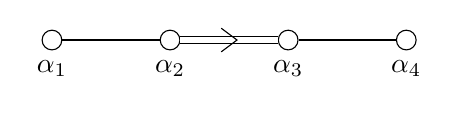
\begin{tikzpicture}[scale=1, baseline=-3pt, circ/.style={draw, circle, inner sep=2pt, minimum size=2.5mm}]
        \node[circ, label=below:$\alpha_1$] (1) at (0,0) {}; 
        \node[circ, label=below:$\alpha_2$] (2) at (1.5,0) {}; 
        \node[circ, label=below:$\alpha_3$] (3) at (3,0) {}; 
        \node[circ, label=below:$\alpha_4$] (4) at (4.5,0) {};
        \draw (1)--(2) (3)--(4);
        \draw[dashed] (2)--(3);
        \draw[double, double distance=2pt] (2) -- (3);
        \draw (2.15,0.15) -- (2.35,0) -- (2.15,-0.15);% Arrow
    \end{tikzpicture}
\end{center}
We denote by $\alpha_0$ and $\alpha^0$ the highest short root and highest long root of the root system, respectively, so the simple affine roots of $G$ are $S_{\aff}=\{-\calpha_0,\calpha_4,\calpha_3,\calpha_2,\calpha_1\}$ with affine Dynkin diagram 
\begin{center}
    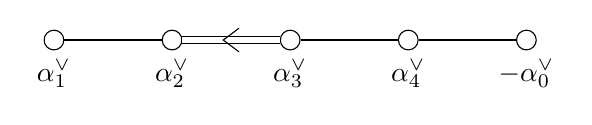
\begin{tikzpicture}[
        circ/.style={draw, circle, inner sep=2pt, minimum size=2.5mm}
    ]
        \node[circ, label=below:$\alpha^\vee_1$] (1) at (0,0) {};
        \node[circ, label=below:$\alpha^\vee_2$] (2) at (1.5,0) {};
        \node[circ, label=below:$\alpha^\vee_3$] (3) at (3,0) {};
        \node[circ, label=below:$\alpha^\vee_4$] (4) at (4.5,0) {};
        \node[circ, label=below:$-\alpha^\vee_0$] (0) at (6,0) {};

        \draw (1) -- (2);
        \draw[double, double distance=2pt] (3) -- (2);
        \draw (3) -- (4);
        \draw (4) -- (0);
        \draw (2.35,0.15) -- (2.15,0) -- (2.35,-0.15);% Arrow
    \end{tikzpicture}
\end{center}

The group $G$ has five maximal open compact subgroups $\{K_0,K_4,K_3,K_2,K_1\}$ up to conjugacy, where $K_i$ corresponds to $J_i:=S_{\aff}\setminus\{\alpha^\vee_i\}$ for $0\leq i\leq 4$. The reductive quotients $\overline{K}_0,\overline{K}_4,\overline{K}_3,\overline{K}_2$ and $\overline{K}_1$ are finite reductive groups of type $F_4, A_1\times C_3, A_2\times\tilde{A}_2, A_3\times\tilde{A}_1$ and $B_4$, respectively. In this section, we prove the following.

\begin{theorem}\label{thm:F4}
    Let $G$ be a simple p-adic group of type $F_4$. Then the diagram 
    \[
        \begin{tikzcd}
            R_{\un,\mathrm{ell}}(G) \arrow[r, "\FT^\vee_{\mathrm{ell}}"] \arrow[d, "\res_{\un}^{\mathrm{cpt}}"] & R_{\un,\mathrm{ell}}(G) \arrow[d, "\res_{\un}^{\mathrm{cpt}}"] \\
            \bigoplus_{i=0}^5 R_{\un}(\overline{K}_i) \arrow[r, "(\FT^{K_i})_i"] & \bigoplus_{i=0}^5 R_{\un}(\overline{K}_i),
        \end{tikzcd}
    \]
    commutes.
\end{theorem}

We remark that the above result was already proven by Ciubotaru, in an unpublished paper \cite{Ciubotaru2020} for the reduction to the hyperspecial parahoric subgroup $K_0$. We complete the proof for the remaining $4$ parahoric subgroups.

Firstly, we compute the basis $\{\Pi(u,s,h)\ |\ u\in G^\vee\text{ unipotent, } (s,h)\in\Gamma_u\backslash\mathcal{Y}(\Gamma_u)_{\mathrm{ell}}\}$ of the space $R_{\un,\text{ell}}(G)$ (see Section \ref{subsec:Fourier_transform} for the definitions). The classification of all elliptic pairs of $F_4(\CC)$ has been previously computed in the literature, and the list is given in Table \ref{tbl:F4_pairs}. For each unipotent $u\in F_4(\CC)$, we also give the unipotent $F_4(\FF_q)$-family $\mathcal{F}_u$ whose special element is the $W$-representation afforded by $\varepsilon\otimes H^{\mathrm{top}}(\mathcal{B}^u)^{\mathbf{1}}$ under the Springer correspondence. Then $\Gamma_{\mathcal{F}_u}$ is the finite group canonically associated to the family $\mathcal{F}_u$.

\begin{table}[ht]
    \centering
    \begin{tabular}{|c|c|c|c|c|c|}
        \hline
        Unipotent & $\Gamma_u^0$ & $A_u$ & $|\Gamma_u\backslash\mathcal(\Gamma_u)_{\text{ell}}|$ & $\mathcal{F}_{u}$ & $\Gamma_{\mathcal{F}_u}$ \\\hline
        $F_4$ & $1$ & $1$ & $1$ & $\phi_{1,24}$ & $1$ \\\hline
        $F_4(a_1)$ & $1$ & $S_2$ & $4$ & $\phi_{4,13}$ & $C_2$ \\\hline
        $F_4(a_2)$ & $1$ & $S_2$ & $4$ & $\phi_{9,10}$ & $1$ \\\hline
        $B_3$ & $\text{PGL}(2)$ & $1$ & $1$ & $\phi_{8,9}''$ & $1$ \\\hline
        $F_4(a_3)$ & $1$ & $S_4$ & $21$ & $\phi_{12,4}$ & $S_4$\\\hline
    \end{tabular}
    \caption{Elliptic pairs for $F_4$}
    \label{tbl:F4_pairs}
\end{table}

In particular, $E_{\un,\text{ell}}(G)$ is a $31$-dimensional vector space, where $21$ of these dimensions come from the distinguished unipotent class $F_4(a_3)$. The proof of Theorem \ref{thm:F4} relies on an explicit computation of the restriction map 
$$\res^{\mathrm{par}}_{\un}:\mathcal{R}_{\un,\mathrm{ell}}^p(G)\longrightarrow\bigoplus_{i=0}^5 R_{\un}(\overline{K}_i).$$
Most of this work was completed by Reeder in \cite{Reeder2000}. Nevertheless, his tables contain a few mistakes (systematically arising from the two representations $\pi(F_4(a_3),1,31)$ and $\pi(F_4(a_3),1,211)$) and do not include the representations whose unipotent label $u$ has type $B_3$ (for this is not a distinguished unipotent element of $F_4(\CC)$). We tabulate these results at the end of the section, fixing the mistakes and adding the new restrictions.

\iffalse To display this information for all unipotent classes simultaneously, we use the notation for the Langlands parameters as in \cite{Reeder2000}, which we now explain for convenience. 

\textbf{Notation:} Given a representation $\pi(x,\phi)$, let $x=us$ be the Jordan decomposition. Then $u\in Z_{G^\vee}(s)^0$ is a unipotent element of the connected pseudo-Levi subgroup $Z_{G^\vee}(s)^0$, and $\phi$ is an irreducible representation of the component group $A_{su}$. The representation $\pi(x,\phi)$ will be labelled by the type of unipotent element $u$ is inside $Z_{G^\vee}(s)^0$, together with the representation $\phi$. For example, if $u$ has type $F_4(a_3)$ and $s$ is a two-cycle, then $Z_{G^\vee}(s)$ has type $C_3\times A_1$, $u$ is labelled by $C_3(42)\times A_1$ (subregular in the first group and regular in the second) and $\widehat{A_{su}}=C_2\times C_2$. Thus, each representation has a name of the form $[u\in Z_{G^\vee}(s)^0,\phi]$ where $\phi$ is an irreducible representation of $A_{su}$.\fi

Let us briefly discuss how the parahoric restrictions are computed. The unipotent representations of $F_4(F)$ fall into $9$ unipotent blocks, together with their associated Hecke algebras. There are $7$ supercuspidal blocks, one for each cuspidal unipotent representation of $F_4(\FF_q)$. The corresponding Hecke algebras $\cH(F_4(F),F_4(\mathcal{O}_F),\sigma)$ are all isomorphic to $\CC$ so these blocks contain a unique unipotent representation. This information can be read from Lusztig's arithmetic-geometric correspondence tables in \cite{Lusztig1995}*{pg. 577}. The Langlands parameters of these representations are $$[F_4(a_3),1^4],\ [C_3(42),--],\ [B_4(531),\varepsilon],\ [2A_2,\theta],\ [2A_2,\theta^2],\ [A_1A_3,i]\text{ and }[A_1A_3,-i],$$
where we are using Notation \ref{notation:Langlandsparam} for the Langlands parameters. The parahoric restrictions of these representations are straightforward to compute, for they are irreducible for the hyperspecial parahoric $K_0$ and vanish for the other ones.

The principal block contains all Iwahori-spherical representations, that is, all representations $\pi(us,\phi)$ such that $H(\mathcal{B}_s^u)^{\phi}\neq 0$. The corresponding Hecke algebra $\cH(F_4(F),I,\mathbf{1})$ is the affine Hecke algebra of type $F_4$ with equal parameters. We compute the parahoric restrictions, using Springer theory, the Green tables of $F_4(\FF_q)$ and the methods described in subsection \ref{subsec:Iwahori_spherical}.

%The parahoric restrictions to the maximal hyperspecial $K_0$ are computed using Springer theory and the Green functions of $F_4(\FF_q)$, which are explicitly known thanks to the work of Beynon-Spaltenstein in \textcolor{red}{Cite BeynonSpaltenstein1984}. The results are tabulated at the end of the section. To compute the parahoric restrictions to the other maximal parahoric subgroups, we use \eqref{eqn:mackey_generalcase}, which relies on the computation of the groups $W_{J,t}$ and the characters $\chi_t^J$. In many instances, the characters are trivial (for example, if $W_{J,t}$ is a reflection subgroup of $W_J$); when this is the case, we use Lemma \ref{lem:mackey_restriction}. The restriction can then be easily obtained from Alvis' tables \textcolor{red}{Insert the reference here}.

Finally, there is an intermediate block whose Hecke algebra $\cH(F_4(F),B_2,\sigma)$ is the affine Hecke algebra of type $C_2$ with unequal parameters that we introduced in Example \ref{ex:F4_B2_algebra}. All Langlands parameters of the representations of interest in this block are \textit{elliptic}, so it suffices to compute the square integrable representations of $\cH(F_4(F),B_2,\sigma)$ to determine the desired parahoric restrictions. This can be achieved using the theory of weight diagrams briefly discussed in Section \ref{sec:weight_diagram} (see also \cite{Ciubotaru2020}*{\S 9}). The Langlands parameters of these representations are $$[B_4,-],\ [C_3A_1,-],\ [C_3(42)A_1,-+],\ [B_4(531),r] \text{ and } [A_1A_3,-1].$$ 
We explicitly discuss the $[A_1A_3,-1]$ case in Example \ref{ex:A1A3}, and we tabulate the rest of the parahoric restrictions at the end of the section.

Before displaying the tables, let us discuss a few examples in detail to illustrate the main ideas involved in the calculations. We will focus on the representations whose unipotent part has type $F_4(a_3)$, since they are the most interesting. 

\subsection{Examples of parahoric restrictions}
The first example is the computation of a parahoric restrictions with respect to the maximal hyperspecial parahoric $K_0$ using Springer Theory and Alvis' tables.

\begin{example}
    Consider the representation $[B_4(531),\mathbf{1}]$, with $u$ of type $F_4(a_3)$ and $s\in\Gamma_u$ a product of two $2$-cycles. The centralizer $Z_{G^\vee}(s)$ has type $B_4$ and $u\in Z_{G^\vee}(s)$ is subregular. Thus, the Springer fibre $\cB^u_s$ is $2$ dimensional, and by reading the Green functions we obtain
    $$H^*(\cB^u_s)^\mathbf{1}=[2,2]+[3,1]+[4,\cdot]\quad\text{as $W_s$-modules}.$$
    Since all characters are trivial when $J=J_0$, Alvis' tables yield
    $$\Ind_{W_s}^W[2,2]+[3,1]+[4,\cdot]=\phi_{9,2}+\phi_{9,6}''+\phi_{8,3}''+\phi_{4,1}+\phi_{2,4}''+\phi_{1,0}.$$
    To obtain the parahoric restriction of the representation $[B_4(531),\mathbf{1}]$ with respect to $K_0$, we twist by $\varepsilon$ and by the outer automorphism of $W$ swapping long and short roots, so
    $$[B_4(531),\mathbf{1}]\xrightarrow{\res^{K_0}_{\un}}\phi_{9,10}+\phi_{9,6}''+\phi_{8,9}''+\phi_{4,13}+\phi_{2,16}''+\phi_{1,24}.$$
\end{example}
Once the parahoric restrictions for the maximal hyperspecial have been calculated, we can turn our attention towards computing the rest. The first step is to determine when the characters $\chi_t^J$ are trivial. The order of the semisimple elements $s$ in the Langlands parameters are clear, while one can show that $Z_{J_1},Z_{J_2},Z_{J_3}$ and $Z_{J_4}$ have order $2,2,3$ and $2$, respectively. Whenever the orders of $s$ and $J_1$ are relatively prime the characters are trivial, and we can use Lemma \ref{lem:mackey_restriction} and Alvis' tables to compute the restriction directly. Let us discuss another interesting example.

\begin{example}
    Consider the parahoric restriction of the Iwahori-spherical representation $[A_1A_3,\mathbf{1}]$, where $u$ is of type $F_4(a_3)$ and $s\in\Gamma_u$ is a $4$-cycle, with respect to the parahoric subgroup $K_2$. Note that $W_{J_2}=\langle s_0,s_4,s_3,s_1\rangle\cong W(A_3)\times W(A_1)$. The semisimple part $s$ can be chosen to be $s=\calpha_3(-1)\calpha_4(i)$ so that $W_s=\langle s_4,s_2,s_1,s^0\rangle\cong W(A_1)\times W(A_3)$. In addition, $u$ is a regular unipotent element in $Z_{G^\vee}(s)$, so $H^*(\mathcal{B}_s^u)^{\mathbf{1}}=\mathbf{1}$ as a $W_s$-module. Next,
    $$W_s\backslash W/W_{J_2}=\{1,w\},$$
    where $w\in W$ is explicitly computable with computer algebra programs such as GAP. In addition, 
    $$W_{J_2,s}=\langle s_4,s_1\rangle\cong C_2\times C_2,\quad\text{while}\quad W_{J_2,s^w}=\langle d \rangle\cong C_4,$$
    for some $d\in W$ of order $4$. Since $W_{J_2,s}$ is a reflection subgroup of $W_{J_2}$, the character $\chi_s^{J_2}$ is trivial. On the other hand, $W_{J_2,s^w}$ is not a reflection subgroup of $W_{J_2}$, and $\chi_{s^w}^{J_2}=\chi$ is a primitive character of $C_4$. The induced representations are then given by
    \begin{align*}
        \Ind_{W_{J_2,s}}^{W_{J_2}}\mathbf{1}=[[4]+2[311]+[22]+[211]]\boxtimes[2]\quad\text{and}\quad\Ind_{W_{J_2,s^w}}^{W_{J_2}}\chi=[[31]+[211]]\boxtimes[[2]+[11]].
    \end{align*}    
    Adding these and twisting by sign gives the required parahoric restriction.
\end{example}



\begin{example}
    A more challenging example is the calculation of the parahoric restriction of $[2A_2,\mathbf{1}]$, with $u$ of type $F_4(a_3)$ and $s\in\Gamma_u$ is a $3$-cycle, with respect to $K_3$. This is the only case where a characters $\chi_{s^w}^{J_3}$ may be non-trivial. Note that $W_{J_3}=\langle s_0,s_4,s_2,s_1\rangle\cong W(A_2)\times W(A_2)$.
    The semisimple part can be taken to be $s=\calpha_3(\xi_3)\calpha_4(\xi_3^2)$, where $\xi_3$ is a primitive third root of unity. In particular, $Z_{G^\vee}(s)$ is a pseudo-Levi subgroup of type $A_2\times A_2$ generated by the affine simple roots $\{\alpha_4,\alpha_3,\alpha_1,-\alpha^0\}$ and $W_s=\langle s_4,s_3,s_1,s^0\rangle$. In addition, the unipotent element $u$ is regular in $Z_{G^\vee}(s)$, so $H^*(\cB^u_s)^{\mathbf{1}}=\mathbf{1}$ as $W_s$-modules. Next,
    $$W_s\backslash W/W_{J_3}=\{w_1=1,w_2,w_3,w_4,w_5\},$$
    where $w_i\in W$ are representatives of double cosets with sizes $324, 324, 36, 36$ and $432$, respectively. The subgroups 
    $$W_{J_3,s^{w_3}}=W_{J_3,s^{w_4}}=W_{J_3}\quad\text{and}\quad W_{J_3,s}\cong W_{J_3,s^{w_2}}\cong C_2\times C_2$$
    are all reflections subgroups of $W_{J_3}$, so the characters $\chi_{s^{w_i}}^{J_3}$ are trivial for $i=1,2,3,4$. The remaining coset is more interesting since    
    $$W_{J_3,s^{w_5}}=\langle d \rangle\cong C_3,$$
    is no longer a reflection subgroup, and $\chi_{s^{w_4}}^{J_3}$ is a primitive character $\chi$ of $C_3$. 
    
    The induced representations are then given by
    \begin{align*}
        \Ind_{W_{J_3,s}}^{J_3}\mathbf{1}=\Ind_{W_{J_3,s^{w_2}}}^{J_3}\mathbf{1}=&[3,3]+[3,21]+[21,3]+[21,21],\quad\Ind_{W_{J_3,s^{w_3}}}^{J_3}\mathbf{1}=\Ind_{W_{J_3,s^{w_4}}}^{J_3}\mathbf{1}=[3,3]\\
        \text{and}\quad&\Ind_{W_{J_3,s^{w_5}}}^{J_3}\chi=[21,3]+[3,21]+[21,21]+[21,1^3]+[1^3,21].
    \end{align*}
    Adding these and twisting by sign gives the required parahoric restriction.
\end{example}

Finally, let us discuss the parahoric restrictions of the non-Iwahori-spherical representation $[A_1A_3,-1]$.

\begin{example}\label{ex:A1A3}
    Let $V$ be the representation labelled by $[A_1A_3,-1]$, $K$ a parahoric subgroup of type $B_2$ and let $\sigma$ be the unique cuspidal unipotent representation of $B_2(\FF_q)$. Since the types of the reductive quotients of $K_2$ and $K_3$ ($A_3\times\tilde{A}_1$ and $A_2\times\tilde{A}_2$, respectively) do not contain $B_2$ as a factor, the parahoric restrictions of $V$ to $K_2$ and $K_3$ vanish. 

    On the other hand, $V^\sigma$ is a square integrable representation of $\cH(F_4(F),B_2,\sigma)\cong\cH(K_{J_0},K,\sigma)\tilde\otimes\mathcal{O}[\mathbf{T}]$, whose restriction to $\mathcal{O}[\mathbf{T}]$ is
    $$V^\sigma|_{\mathcal{O}[\mathbf{T}]}=V^\sigma(q^{-2},-q^{-1})\oplus V^\sigma(-q^{-1},q^{-2}),$$
    both subspaces being one-dimensional. By choosing a basis element in each subspace, the rational functions $e_{\alpha_1}, e_{\alpha_2}\in\mathcal{O}[\mathbf{T}]$ act on $V^\sigma$ by $\mathrm{diag}(-q^{-1},-q)$ and $\mathrm{diag}(-q^{-1},q^{-2})$. Using the formula for the twisted multiplication in $\cH(F_4(F),B_2,\sigma)$, the action of the generators $T_1$ and $T_2$ can be computed explicitly, and we obtain
    \begin{equation*}
        T_{s_1}\longrightarrow\frac{1}{q+1}\begin{pmatrix}
            q^3-1 & q^3+q \\
            q^4+1 & q^4-q
        \end{pmatrix}\quad\text{and}\quad T_{s_2}\longrightarrow\begin{pmatrix}
            -1 & 0 \\
            0 & -1
        \end{pmatrix}.
    \end{equation*}
    Finally, one can trace back through the isomorphisms $\cH(F_4(F),B_2,\sigma)\cong\cH(K_{J_0},K,\sigma)\ \tilde\otimes\ \mathcal{O}[\mathbf{T}]$ to obtain that $T_{\tilde{s}_0}$ acts by
    \begin{equation*}
        T_{\tilde{s}_0}\longrightarrow\frac{1}{q^3+q^2}\begin{pmatrix}
            -q^6+q^3-q^2-1 & q^5+q^3-q^2-1 \\
            -q^7+q^4-q^3+1 & q^6+q^4-q^3+1
        \end{pmatrix}.
    \end{equation*}
    Thus, the action of $\tilde{W}(K,\sigma)$ on $V^\sigma_{q=1}$ is given by
    \begin{equation*}
        s_1\longrightarrow\begin{pmatrix}
            0 & 1 \\
            1 & 0
        \end{pmatrix},\quad s_2\longrightarrow\begin{pmatrix}
            -1 & 0 \\
            0 & -1
        \end{pmatrix}\quad\text{and}\quad \tilde{s}_0\longrightarrow\begin{pmatrix}
            -1 & 0 \\
            0 & 1
        \end{pmatrix}.
    \end{equation*}
    The parahoric restrictions are now obtained by restricting to reflection subgroups. Restriction to the reflection subgroup $\langle s_1,s_2\rangle\cong W(B_2)$ gives the parahoric restriction to $K_0$, restriction to $\langle s_1,\tilde{s}_0\rangle\cong W(B_2)$ gives the parahoric restriction to $K_1$ and restriction to $\langle s_2,\tilde{s}_0\rangle\cong W(A_1\times A_1)$ gives the parahoric restriction to $K_4$. In each case, there is a bijection between representations of the Weyl group and unipotent representations of $\overline{K}_i$ in the series generated by $\sigma$, which we use implicitly. Throughout, we use Lusztig's notation for the unipotent representations. We obtain
    \begin{itemize}
        \item Firstly, $V^\sigma|_{\langle s_1,s_2\rangle}=[11,\emptyset]+[\emptyset,11]$, so $[A_1A_3,-1]\xrightarrow{\res^{K_0}_{\un}}B_2[\varepsilon']+B_2[\varepsilon].$
        \item Secondly, $V^\sigma|_{\langle s_1,\tilde{s}_0\rangle}=[1,1]$, so $[A_1A_3,-1]\xrightarrow{\res^{K_1}_{\un}}\begin{psmallmatrix}
            0 \ 1\ 2\ 4\\
            \ \ \ 1 \ \ \
        \end{psmallmatrix}$.
        \item Finally, $V^\sigma|_{\langle s_2,\tilde{s}_0\rangle}=[11]\boxtimes[2]+[11]\boxtimes[11]$, so $[A_1A_3,-1]\xrightarrow{\res^{K_4}_{\un}}\begin{psmallmatrix}
            0 \ 1\ 2\ 3\\
            \ \ \ 1 \ \ \
        \end{psmallmatrix}\boxtimes\mathbf{1}+\begin{psmallmatrix}
            0 \ 1\ 2\ 3\\
            \ \ \ 1 \ \ \
        \end{psmallmatrix}\boxtimes\St.$
    \end{itemize}
\end{example}


\iffalse

For the purposes of this document, we will instead just discuss in detail a few examples that already highlight the main ideas involved in the calculation for distinct parahoric subgroups $K_i$. All examples discussed come from Iwahori-spherical representations, since the parahoric restrictions of the other representations are still work in progress. This work was mostly completed by \cite[\S 10]{Reeder2000}, but his tables contain some mistakes, systematically arising from the two representations $\pi(F_4(a_3),1,31)$ and $\pi(F_4(a_3),1,211)$. We have been unable to guess where the mistake may have come from. We gather all the results in large tables at the end of the section that fix the mistakes in Reeder's tables. We omit the tables for the parahoric restriction to maximal hyperspecial for a few reasons; they take the most space, the are already correct in Reeder's paper (except for the restriction of $[B_4(531),\epsilon'']$, where the second $K_0$ type should be $\phi_{2,16}'$ instead of $\phi_{2,16}''$) and Theorem \ref{thm:F4} has already been proven in this case.

The conjecture can be verified one unipotent class $u\in G^\vee$ at a time. By far, the most interesting case is the class $F_4(a_3)$, so all examples will involve representations labelled by this class. Let us introduce some helpful notation used in \cite{Reeder2000}. The class $F_4(a_3)$ is distinguished with component group isomorphic to $S_4$, so there are $5$ conjugacy classes of semisimple elements commuting with any $u\in F_4(a_3)$. If $s$ is such a semisimple element, then $Z_{G^\vee}(s)$ is a pseudo-Levi subgroup of a certain type, and $u$ is a unipotent element of this group with a certain label. Then the representation of $F_4(F)$ parametrized by $(us,\phi),\phi\in\widehat{A_{su}}$ will be labelled by the type of unipotent $u$ inside $Z_{G^\vee}(s)$, together with the representation $\phi$.

For example, if $s$ is a two-cycle, then $Z_{G^\vee}(s)$ has type $C_3\times A_1$, $\widehat{A_{su}}=C_2\times C_2$ and $u$ is labelled by $C_3(42)\times A_1$ (subregular in the first group and regular in the second). If $s$ is a three-cycle, then $Z_{G^\vee}(s)$ has type $A_2\times A_2$, $\widehat{A_{su}}$ and $u$ is a regular unipotent labelled by $2A_2$. See the tables at the end for all the labels.

\fi
\newpage
\section{Parahoric restriction tables}
Let us clarify some of the notation used in the tables below. We use the notation described in \ref{notation:Langlandsparam} for the Langlands labels parametrizing the unipotent representations of $G=F_4(F)$. This is the same notation used in Reeder's tables \cite{Reeder2000}. The unipotent representations of finite reductive groups of Lie type are labelled as follows. For groups of type $A_n$, they are parametrized by partitions $\lambda$ of $n+1$. For groups of type $B_n/C_n$, the principal series representations are parametrized by double partitions $[\lambda,\mu]$ of $n$. To understand these tables, it is enough to know that groups of type $B_3/C_3$ have two non-principal series representations $\theta_1$ and $\theta_2$, while groups of type $B_4/C_4$ have five non-principal series representations $\theta_1,\ldots,\theta_5$. They all lie in the same representation series, arising from the unipotent cuspidal representation of their Levi subgroup of type $B_2/C_2$.


\subsection{Parahoric restriction tables for \texorpdfstring{$F_4$}{PDFstring}}
For every parahoric subgroup $K_i$, we present two tables. The first one is the table of parahoric restrictions for all Iwahori-spherical representations of $F_4(F)$ of interest. The second table contains the parahoric restrictions of all virtual characters $\Pi(u,s,h)$, where representations of $\overline{K}_i$ are organized in terms of the families. Firstly, we write the characters in trivial families; then we write each family, with the special character always coming first. We omit the tables for the maximal hyperspecial parahoric subgroup $K_0$, for the restrictions can be found in \cite{Reeder2000}[\S 10], and the conjecture has already been verified in \cite{Ciubotaru2020}. In particular, all nontrivial families $\mathcal{U}$ that appear in the tables have size $4$, with corresponding group $\Gamma_\mathcal{U}=C_2$, so Lusztig's non-abelian Fourier transform acts by 
$$\begin{pmatrix}
    \frac{1}{2} & \frac{1}{2} & \frac{1}{2} & \frac{1}{2} \\
    \frac{1}{2} & \frac{1}{2} & -\frac{1}{2} & -\frac{1}{2} \\
    \frac{1}{2} & -\frac{1}{2} & \frac{1}{2} & -\frac{1}{2} \\
    \frac{1}{2} & -\frac{1}{2} & -\frac{1}{2} & \frac{1}{2} 
\end{pmatrix}.$$

From these tables, the statement of Theorem \ref{thm:F4} can be easily verified using Lusztig's nonabelian transform. For reference, we write here the virtual characters $\Pi(u,s,h)$ in terms of representations of $F_4(F)$ when $u\in F_4(a_3)$. In the notation below, $\tau=g_2\cdot g_2'$ is another $2$-cycle conjugate to $g_2$ in $A_u=S_4$ but not in $A_{ug_2}=C_2\times C_2$ and, similarly, $\gamma$ is an element conjugate to $g_2'$ in $A_u=S_4$ but not in $A_{ug_2'}=D_8$. The analogous expressions for other unipotent classes are much simpler. 

\begin{align*}
    \Pi(u,1,1)&= [F_4(a_3),4] + 3[F_4(a_3),31] + 3[F_4(a_3),211] + [F_4(a_3),1^4] + 2[F_4(a_3),22]; \\
    \Pi(u, 1, g_2) &= [F_4(a_3),4] + [F_4(a_3),31] - [F_4(a_3),211] - [F_4(a_3),1^4]; \\
    \Pi(u, 1, g_2') &= [F_4(a_3),4] - [F_4(a_3),31] - [F_4(a_3),211] + [F_4(a_3),1^4] + 2[F_4(a_3),22]; \\
    \Pi(u, 1, g_3) &= [F_4(a_3),4] + [F_4(a_3),1^4] - [F_4(a_3),22]; \\
    \Pi(u, 1, g_4) &= [F_4(a_3),4] - [F_4(a_3),31] + [F_4(a_3),211] - [F_4(a_3),1^4]; 
\end{align*}
\begin{align*}
    \Pi(u, g_2, 1) &= [C(42)A_1,++] + [C(42)A_1,+-] + [C(42)A_1,-+] + [C(42)A_1,--]; \\
    \Pi(u, g_2, g_2) &= [C(42)A_1,++] - [C(42)A_1,+-] + [C(42)A_1,-+] - [C(42)A_1,--]; \\
    \Pi(u, g_2, \tau) &= [C(42)A_1,++] + [C(42)A_1,+-] - [C(42)A_1,-+] - [C(42)A_1,--]; \\
    \Pi(u, g_2, g_2') &= [C(42)A_1,++] - [C(42)A_1,+-] - [C(42)A_1,-+] + [C(42)A_1,--]; 
\end{align*}
\begin{align*}
    \Pi(u,g_2',1) &= [B_4(531),\mathbf{1}] + 2[B_4(531),r] + [B_4(531),\varepsilon'] + [B_4(531),\varepsilon''] + [B_4(531),\varepsilon]; \\
    \Pi(u, g_2', g_2') &= [B_4(531),\mathbf{1}] - [B_4(531),\varepsilon'] + [B_4(531),\varepsilon''] - [B_4(531),\varepsilon]; \\
    \Pi(u, g_2', g_2'') &= [B_4(531),\mathbf{1}] - 2[B_4(531),r] + [B_4(531),\varepsilon'] + [B_4(531),\varepsilon''] + [B_4(531),\varepsilon]; \\
    \Pi(u, g_2', g_4) &= [B_4(531),\mathbf{1}] - [B_4(531),\varepsilon'] - [B_4(531),\varepsilon''] + [B_4(531),\varepsilon]; \\
    \Pi(u, g_2', \gamma) &= [B_4(531),\mathbf{1}] + [B_4(531),\varepsilon'] - [B_4(531),\varepsilon''] - [B_4(531),\varepsilon];
\end{align*}
\begin{align*}
    \Pi(u, g_3, 1) &= [2A_2,\mathbf{1}] + [2A_2,\theta] + [2A_2,\theta^2]; \\
    \Pi(u, g_3, g_3) &= [2A_2,\mathbf{1}] + \theta^2[2A_2,\theta] + \theta[2A_2,\theta^2]; \\
    \Pi(u, g_3, g_3^{-1}) &= [2A_2,\mathbf{1}] + \theta[2A_2,\theta] + \theta^2[2A_2,\theta^2];
\end{align*}
\begin{align*}
    \Pi(u, g_4, 1) &= [A_3A_1,1] + [A_3A_1,i] + [A_3A_1,-1] + [A_3A_1,-i]; \\
    \Pi(u, g_4, g_4) &= [A_3A_1,1] - i[A_3A_1,i] - [A_3A_1,-1] - i[A_3A_1,-i]; \\
    \Pi(u, g_4, g_4') &= [A_3A_1,1] - [A_3A_1,i] + [A_3A_1,-1] - [A_3A_1,-i]; \\
    \Pi(u, g_4, g_4^{-1}) &= [A_3A_1,1] + i[A_3A_1,i] - [A_3A_1,-1] - i[A_3A_1,-i];
\end{align*}




\begin{landscape}
    \centering
    \subsubsection*{Iwahori-spherical \texorpdfstring{$B_4$}{PDFstring}-types}
    \begin{table}[ht]
        \centering
        {\small
        \begin{tabular}{|c|cccccccccccc|}
            \hline
            & $[21^2,\cdot]$ & $[1^4,\cdot]$ & $[1^3,1]$ & $[2,11]$ & $[11,2]$ & $[11,11]$ & $[1,21]$ & $[1,1^3]$ & $[\cdot,31]$ & $[\cdot,22]$ & $[\cdot,21^2]$ & $[\cdot,1^4]$ \\\hline
            $[F_4,1]$ & 0 & 0 & 0 & 0 & 0 & 0 & 0 & 0 & 0 & 0 & 0 & 1\\\hline
            $[F_4(a_1),+]$ & 0 & 0 & 0 & 0 & 0 & 0 & 0 & 1 & 0 & 0 & 0 & 1\\
            $[F_4(a_1),-]$ & 0 & 1 & 0 & 0 & 0 & 0 & 0 & 0 & 0 & 0 & 0 & 1\\
            $[B_4,+]$ & 0 & 0 & 0 & 0 & 0 & 0 & 0 & 0 & 0 & 0 & 1 & 0\\\hline
            $[F_4(a_2),+]$ & 0 & 0 & 0 & 0 & 0 & 1 & 0 & 1 & 0 & 0 & 1 & 1\\
            $[F_4(a_2),-]$ & 0 & 0 & 0 & 0 & 0 & 0 & 0 & 0 & 0 & 1 & 0 & 0\\
            $[C_3A_1,+]$ & 0 & 0 & 1 & 0 & 0 & 0 & 0 & 1 & 0 & 0 & 1 & 1\\\hline
            $[B_4(711),+]$ & 0 & 0 & 0 & 0 & 0 & 0 & 1 & 1 & 0 & 0 & 1 & 0\\
            $[B_4(711),-]$ & 0 & 0 & 0 & 0 & 0 & 1 & 0 & 0 & 0 & 1 & 0 & 1\\\hline
            $[F_4(a_3),4]$ & 0 & 0 & 1 & 1 & 1 & 1 & 1 & 2 & 0 & 0 & 1 & 1\\
            $[F_4(a_3),31]$ & 1 & 1 & 1 & 0 & 0 & 1 & 0 & 1 & 0 & 0 & 0 & 1 \\
            $[F_4(a_3),22]$ & 0 & 0 & 0 & 1 & 0 & 0 & 0 & 1 & 0 & 0 & 0 & 0 \\
            $[F_4(a_3),211]$ & 0 & 1 & 0 & 0 & 0 & 0 & 0 & 0 & 0 & 0 & 0 & 0 \\
            $[C_3(42)A_1,++]$ & 1 & 0 & 1 & 1 & 1 & 1 & 1 & 2 & 0 & 0 & 2 & 1 \\
            $[C_3(42)A_1,+-]$ & 0 & 1 & 1 & 0 & 0 & 1 & 0 & 0 & 0 & 0 & 0 & 1 \\
            $[B_4(531),1]$ & 0 & 0 & 0 & 1 & 1 & 0 & 1 & 1 & 1 & 0 & 2 & 0 \\
            $[B_4(531),\varepsilon']$ & 0 & 0 & 0 & 0 & 0 & 0 & 0 & 0 & 1 & 0 & 0 & 0 \\
            $[B_4(531),\varepsilon'']$ & 1 & 0 & 0 & 0 & 0 & 0 & 0 & 0 & 0 & 0 & 1 & 0 \\
            $[2A_2,1]$ & 0 & 0 & 1 & 0 & 1 & 1 & 1 & 1 & 0 & 0 & 1 & 1 \\
            $[A_1A_3,1]$ & 0 & 0 & 0 & 0 & 1 & 0 & 1 & 1 & 1 & 0 & 1 & 0 \\\hline
        \end{tabular}
        }
        \caption{Parahoric restriction of unipotent $F_4(F)$-representations with respect to $K_1$}
    \end{table}
    \iffalse
    \begin{table}[ht]
        \centering
        {\tiny
        \begin{tabular}{|c|ccccc|cccR|cccR|cccR|cccR|}
            \hline
        & $[4,\cdot]$ & $[21,1]$ & $[11,2]$ & $[1,21]$ & $[\cdot,1^4]$ & $[1,1^3]$ & $[1^4,\cdot]$ & $[\cdot,21^2]$ & $\theta_1$ & $[11,11]$ & $[1^3,1]$ & $[\cdot,22]$ & $\theta_2$ & $[2,11]$ & $[21^2,\cdot]$ & $[\cdot,31]$ & $\theta_3$ & $[2,2]$ & $[22,\cdot]$ & $[1,3]$ & $\theta_4$ \\\hline
        $\Pi(u,1,1)$ & 0 & 0 & 1 & 1 & 4 & 7 & 6 & 1 & 0 & 4 & 4 & 0 & 0 & 3 & 3 & 0 & 0 & 0 & 0 & 0 & 0 \\
        $\Pi(u,1,g_2)$ & 0 & 0 & 1 & 1 & 2 & 3 & 0 & 1 & 0 & 2 & 2 & 0 & 0 & 1 & 1 & 0 & 0 & 0 & 0 & 0 & 0 \\
        $\Pi(u,1,g_2')$ & 0 & 0 & 1 & 1 & 0 & 3 & -2 & 1 & 0 & 0 & 0 & 0 & 0 & 3 & -1 & 0 & 0 & 0 & 0 & 0 & 0 \\
        $\Pi(u,1,g_3)$ & 0 & 0 & 1 & 1 & 1 & 1 & 0 & 1 & 0 & 1 & 1 & 0 & 0 & 0 & 0 & 0 & 0 & 0 & 0 & 0 & 0 \\
        $\Pi(u,1,g_4)$ & 0 & 0 & 1 & 1 & 0 & 1 & 0 & 1 & 0 & 0 & 0 & 0 & 0 & 1 & -1 & 0 & 0 & 0 & 0 & 0 & 0 \\\hline
        $\Pi(u,g_2,1)$  & 0 & 0 & 1 & 1 & 2 & 2 & 1 & 2 & 1 & 2 & 2 & 0 & 0 & 1 & 1 & 0 & 0 & 0 & 0 & 0 & 0 \\
        $\Pi(u,g_2,g_2)$ & 0 & 0 & 1 & 1 & 2 & 2 & 1 & 2 & {-1} & 2 & 2 & 0 & 0 & 1 & 1 & 0 & 0 & 0 & 0 & 0 & 0 \\
        $\Pi(u,g_2,\tau)$ & 0 & 0 & 1 & 1 & 0 & 2 & {-1} & 2 & 1 & 0 & 0 & 0 & 0 & 1 & 1 & 0 & 0 & 0 & 0 & 0 & 0 \\
        $\Pi(u,g_2,g_2')$ & 0 & 0 & 1 & 1 & 0 & 2 & {-1} & 2 & {-1} & 0 & 0 & 0 & 0 & 1 & 1 & 0 & 0 & 0 & 0 & 0 & 0 \\\hline
        $\Pi(u,g_2',1)$ & 0 & 0 & 1 & 1 & 0 & 1 & 0 & {3} & 2 & 0 & 0 & 0 & 0 & 1 & 1 & 2 & 2 & 0 & 0 & 0 & 0 \\
        $\Pi(u,g_2',g_2)$ &  0 & 0 & 1 & 1 & 0 & 1 & 0 & {3} & 0 & 0 & 0 & 0 & 0 & 1 & 1 & 0 & 0 & 0 & 0 & 0 & 0 \\
        $\Pi(u,g_2',g_2')$ & 0 & 0 & 1 & 1 & 0 & 1 & 0 & {3} & {-2} & 0 & 0 & 0 & 0 & 1 & 1 & 2 & {-2} & 0 & 0 & 0 & 0 \\
        $\Pi(u,g_2',\gamma)$ & 0 & 0 & 1 & 1 & 0 & 1 & 0 & 1 & 0 & 0 & 0 & 0 & 0 & 1 & {-1} & 2 & 0 & 0 & 0 & 0 & 0 \\
        $\Pi(u,g_2',g_4)$ & 0 & 0 & 1 & 1 & 0 & 1 & 0 & 1 & 0 & 0 & 0 & 0 & 0 & 1 & {-1} & 0 & 0 & 0 & 0 & 0 & 0 \\\hline
        $\Pi(u,g_3,h)$ & 0 & 0 & 1 & 1 & 1 & 1 & 0 & 1 & 0 & 1 & 1 & 0 & 0 & 0 & 0 & 0 & 0 & 0 & 0 & 0 & 0 \\\hline
        $\Pi(u,g_4,1/g_2')$ & 0 & 0 & 1 & 1 & 0 & 1 & 0 & 1 & 0 & 0 & 0 & 0 & 0 & 0 & 0 & 1 & 1 & 0 & 0 & 0 & 0 \\
        $\Pi(u,g_4,g_4^{\pm1})$ & 0 & 0 & 1 & 1 & 0 & 1 & 0 & 1 & 0 & 0 & 0 & 0 & 0 & 0 & 0 & 1 & {-1} & 0 & 0 & 0 & 0 \\\hline
        \end{tabular}
        }
        \caption{Parahoric restrictions of the virtual characters $\Pi(u,s,h)$ where $u\in F_4(a_3)$ with respect to $K_1$}
    \end{table}
    \fi

    \newpage

    \begin{table}[ht]
        \centering
        {\small
        \begin{tabular}{|c|ccc|cccc|cccc|cccc|}
            \hline
            & $[11,2]$ & $[1,21]$ & $[\cdot,1^4]$ & $[1,1^3]$ & $[1^4,\cdot]$ & $[\cdot,21^2]$ & $\theta_1$ & $[11,11]$ & $[1^3,1]$ & $[\cdot,22]$ & $\theta_2$ & $[2,11]$ & $[21^2,\cdot]$ & $[\cdot,31]$ & $\theta_3$ \\\hline
            $\Pi(u,1,1)$ & 1 & 1 & 4 & 7 & 6 & 1 & 0 & 4 & 4 & 0 & 0 & 3 & 3 & 0 & 0 \\
            $\Pi(u,1,g_2)$ & 1 & 1 & 2 & 3 & 0 & 1 & 0 & 2 & 2 & 0 & 0 & 1 & 1 & 0 & 0 \\
            $\Pi(u,1,g_2')$ & 1 & 1 & 0 & 3 & -2 & 1 & 0 & 0 & 0 & 0 & 0 & 3 & -1 & 0 & 0 \\
            $\Pi(u,1,g_3)$ & 1 & 1 & 1 & 1 & 0 & 1 & 0 & 1 & 1 & 0 & 0 & 0 & 0 & 0 & 0 \\
            $\Pi(u,1,g_4)$ & 1 & 1 & 0 & 1 & 0 & 1 & 0 & 0 & 0 & 0 & 0 & 1 & -1 & 0 & 0 \\\hline
            $\Pi(u,g_2,1)$  & 1 & 1 & 2 & 2 & 1 & 2 & 1 & 2 & 2 & 0 & 0 & 1 & 1 & 0 & 0 \\
            $\Pi(u,g_2,g_2)$ & 1 & 1 & 2 & 2 & 1 & 2 & {-1} & 2 & 2 & 0 & 0 & 1 & 1 & 0 & 0 \\
            $\Pi(u,g_2,tau)$ & 1 & 1 & 0 & 2 & {-1} & 2 & 1 & 0 & 0 & 0 & 0 & 1 & 1 & 0 & 0 \\
            $\Pi(u,g_2,g_2')$ & 1 & 1 & 0 & 2 & {-1} & 2 & {-1} & 0 & 0 & 0 & 0 & 1 & 1 & 0 & 0 \\\hline
            $\Pi(u,g_2',1)$ & 1 & 1 & 0 & 1 & 0 & {3} & 2 & 0 & 0 & 0 & 0 & 1 & 1 & 2 & 2 \\
            $\Pi(u,g_2',g_2)$ & 1 & 1 & 0 & 1 & 0 & {3} & 0 & 0 & 0 & 0 & 0 & 1 & 1 & 0 & 0 \\
            $\Pi(u,g_2',g_2')$ & 1 & 1 & 0 & 1 & 0 & {3} & {-2} & 0 & 0 & 0 & 0 & 1 & 1 & 2 & {-2} \\
            $\Pi(u,g_2',\gamma)$ & 1 & 1 & 0 & 1 & 0 & 1 & 0 & 0 & 0 & 0 & 0 & 1 & {-1} & 2 & 0 \\
            $\Pi(u,g_2',g_4)$ & 1 & 1 & 0 & 1 & 0 & 1 & 0 & 0 & 0 & 0 & 0 & 1 & {-1} & 0 & 0 \\\hline
            $\Pi(u,g_3,h)$ & 1 & 1 & 1 & 1 & 0 & 1 & 0 & 1 & 1 & 0 & 0 & 0 & 0 & 0 & 0 \\\hline
            $\Pi(u,g_4,1/g_2')$ & 1 & 1 & 0 & 1 & 0 & 1 & 0 & 0 & 0 & 0 & 0 & 0 & 0 & 1 & 1 \\
            $\Pi(u,g_4,g_4^{\pm1})$ & 1 & 1 & 0 & 1 & 0 & 1 & 0 & 0 & 0 & 0 & 0 & 0 & 0 & 1 & {-1} \\\hline
        \end{tabular}
        }
        \caption{Parahoric restrictions of the virtual characters $\Pi(u,s,h)$ where $u\in F_4(a_3)$ with respect to $K_1$}
    \end{table}

    \centering
    \newpage
    \subsubsection*{Iwahori-spherical \texorpdfstring{$A_3\times A_1$}{PDFstring}-types}
    \iffalse
    \begin{table}[h]
        \centering
        \begin{minipage}{0.40\textwidth}
            \centering
            % --- First table ---
            \begin{tabular}{|c|ccccc|}
                \hline
                & $[1^4]$ & $[211]$ & $[22]$ & $[31]$ & $[4]$ \\\hline
                $[F_4,1]$ & $0,\bar1$ & $0,\bar0$ & $0,\bar0$ & $0,\bar0$ & $0,\bar0$ \\\hline
                $[F_4(a_1),+]$ & $1,\bar1$ & $0,\bar1$ & $0,\bar0$ & $0,\bar0$ & $0,\bar0$ \\
                $[F_4(a_1),-]$ & $1,\bar1$ & $0,\bar0$ & $0,\bar0$ & $0,\bar0$ & $0,\bar0$ \\
                $[B_4,+]$ & $0,\bar0$ & $0,\bar1$ & $0,\bar0$ & $0,\bar0$ & $0,\bar0$ \\\hline
                $[F_4(a_2),+]$ & $1,\bar2$ & $1,\bar2$ & $0,\bar1$ & $0,\bar0$ & $0,\bar0$ \\
                $[F_4(a_2),-]$ & $0,\bar0$ & $0,\bar0$ & $0,\bar1$ & $0,\bar0$ & $0,\bar0$ \\
                $[C_3A_1,+]$ & $1,\bar2$ & $1,\bar2$ & $0,\bar0$ & $0,\bar0$ & $0,\bar0$ \\\hline
                $[B_4(711),+]$ & $0,\bar0$ & $0,\bar0$ & $0,\bar0$ & $0,\bar0$ & $0,\bar0$ \\
                $[B_4(711),-]$ & $0,\bar0$ & $0,\bar0$ & $0,\bar0$ & $0,\bar0$ & $0,\bar0$ \\\hline
                $[F_4(a_3),4]$ & $2,\bar{3}$ & $3,\bar{5}$ & $1,\bar1$ & $1,\bar2$ & $0,\bar0$ \\
                $[F_4(a_3),31]$ & $3,\bar2$ & $2,\bar2$ & $1,\bar0$ & $0,\bar0$ & $0,\bar0$ \\
                $[F_4(a_3),22]$ & $1,\bar0$ & $1,\bar1$ & $0,\bar0$ & $0,\bar1$ & $0,\bar0$ \\
                $[F_4(a_3),211]$ & $1,\bar0$ & $0,\bar0$ & $0,\bar0$ & $0,\bar0$ & $0,\bar0$ \\
                $[C_3(42)A_1,++]$ & $2,\bar{3}$ & $4,\bar{6}$ & $1,\bar1$ & $1,\bar2$ & $0,\bar0$ \\
                $[C_3(42)A_1,+-]$ & $2,\bar2$ & $1,\bar1$ & $1,\bar0$ & $0,\bar0$ & $0,\bar0$ \\
                $[B_4(531),1]$ & $0,\bar1$ & $2,\bar{4}$ & $0,\bar1$ & $1,\bar{3}$ & $0,\bar0$ \\
                $[B_4(531),\varepsilon'']$ & $0,\bar0$ & $1,\bar1$ & $0,\bar0$ & $0,\bar0$ & $0,\bar0$ \\
                $[B_4(531),\varepsilon']$ & $0,\bar0$ & $0,\bar0$ & $0,\bar0$ & $0,\bar1$ & $0,\bar0$ \\
                $[2A_2,1]$ & $1,\bar{3}$ & $2,\bar{4}$ & $1,\bar1$ & $1,\bar1$ & $0,\bar0$ \\
                $[A_1A_3,1]$ & $0,\bar1$ & $1,\bar{3}$ & $0,\bar1$ & $1,\bar2$ & $0,\bar0$ \\\hline
            \end{tabular}
            \caption{\centering{Parahoric restriction of \\ $F_4(F)$-representations labelled by the \\ distinguished unipotent $F_4(a_3)$ with respect to $K_2$}}
        \end{minipage}
        \hfill
        \begin{minipage}{0.40\textwidth}
            \centering
            \begin{tabular}{|c|ccccc|}
                \hline
                & $[1^4]$ & $[211]$ & $[22]$ & $[31]$ & $[4]$ \\\hline
                $\Pi(u,1,1)$ & $16,\bar{9}$ & $11,\bar{13}$ & $4,\bar1$ & $1,\bar{4}$ & $0,\bar0$ \\
                $\Pi(u,1,g_2)$ & $4,\bar{5}$ & $5,\bar{7}$ & $2,\bar1$ & $1,\bar2$ & $0,\bar0$ \\
                $\Pi(u,1,g_2')$ & $0,\bar1$ & $3,\bar{5}$ & $0,\bar1$ & $1,\bar{4}$ & $0,\bar0$ \\
                $\Pi(u,1,g_3)$ & $1,\bar{3}$ & $2,\bar{4}$ & $1,\bar1$ & $1,\bar1$ & $0,\bar0$ \\
                $\Pi(u,1,g_4)$ & $0,\bar1$ & $1,\bar{3}$ & $0,\bar1$ & $1,\bar2$ & $0,\bar0$ \\\hline
                $\Pi(u,g_2,1)$ & $4,\bar{5}$ & $5,\bar{7}$ & $2,\bar1$ & $1,\bar2$ & $0,\bar0$ \\
                $\Pi(u,g_2,g_2)$ & $4,\bar{5}$ & $5,\bar{7}$ & $2,\bar1$ & $1,\bar2$ & $0,\bar0$ \\
                $\Pi(u,g_2,\tau)$ & $0,\bar1$ & $3,\bar{5}$ & $0,\bar1$ & $1,\bar2$ & $0,\bar0$ \\
                $\Pi(u,g_2,g_2')$ & $0,\bar1$ & $3,\bar{5}$ & $0,\bar1$ & $1,\bar2$ & $0,\bar0$ \\\hline
                $\Pi(u,g_2',1)$ & $0,\bar1$ & $3,\bar{5}$ & $0,\bar1$ & $1,\bar{4}$ & $0,\bar0$ \\
                $\Pi(u,g_2',g_2)$ & $0,\bar1$ & $3,\bar{5}$ & $0,\bar1$ & $1,\bar2$ & $0,\bar0$ \\
                $\Pi(u,g_2',\gamma)$ & $0,\bar1$ & $1,\bar{3}$ & $0,\bar1$ & $1,\bar4$ & $0,\bar0$ \\
                $\Pi(u,g_2',g_2')$ & $0,\bar1$ & $3,\bar{5}$ & $0,\bar1$ & $1,\bar4$ & $0,\bar0$ \\
                $\Pi(u,g_2',g_4)$ & $0,\bar1$ & $1,\bar{3}$ & $0,\bar1$ & $1,\bar2$ & $0,\bar0$ \\\hline
                $\Pi(u,g_3,h)$ & $1,\bar{3}$ & $2,\bar{4}$ & $1,\bar1$ & $1,\bar1$ & $0,\bar0$ \\\hline
                $\Pi(u,g_4,h)$ & $0,\bar1$ & $1,\bar{3}$ & $0,\bar1$ & $1,\bar2$ & $0,\bar0$ \\\hline
            \end{tabular}
            \caption{\centering{Parahoric restrictions of the virtual characters $\Pi(u,s,h)$ where $u\in F_4(a_3)$ \\ with respect to $K_2$}}
        \end{minipage}
    \end{table}
    \newpage
    \fi
    \begin{table}[h]
        \centering % This centers the entire block of two minipages
        
        % Reduced width to 0.35 or 0.30 so they don't fight for space
        \begin{minipage}{0.4\textwidth}
            \centering
            \begin{tabular}{|c|ccccc|}
                \hline
                & $[1^4]$ & $[211]$ & $[22]$ & $[31]$ & $[4]$ \\\hline
                $[F_4,1]$ & $0,\bar1$ & $0,\bar0$ & $0,\bar0$ & $0,\bar0$ & $0,\bar0$ \\\hline
                $[F_4(a_1),+]$ & $1,\bar1$ & $0,\bar1$ & $0,\bar0$ & $0,\bar0$ & $0,\bar0$ \\
                $[F_4(a_1),-]$ & $1,\bar1$ & $0,\bar0$ & $0,\bar0$ & $0,\bar0$ & $0,\bar0$ \\
                $[B_4,+]$ & $0,\bar0$ & $0,\bar1$ & $0,\bar0$ & $0,\bar0$ & $0,\bar0$ \\\hline
                $[F_4(a_2),+]$ & $1,\bar2$ & $1,\bar2$ & $0,\bar1$ & $0,\bar0$ & $0,\bar0$ \\
                $[F_4(a_2),-]$ & $0,\bar0$ & $0,\bar0$ & $0,\bar1$ & $0,\bar0$ & $0,\bar0$ \\
                $[C_3A_1,+]$ & $1,\bar2$ & $1,\bar2$ & $0,\bar0$ & $0,\bar0$ & $0,\bar0$ \\\hline
                $[B_4(711),+]$ & $0,\bar0$ & $0,\bar0$ & $0,\bar0$ & $0,\bar0$ & $0,\bar0$ \\
                $[B_4(711),-]$ & $0,\bar0$ & $0,\bar0$ & $0,\bar0$ & $0,\bar0$ & $0,\bar0$ \\\hline
                $[F_4(a_3),4]$ & $2,\bar{3}$ & $3,\bar{5}$ & $1,\bar1$ & $1,\bar2$ & $0,\bar0$ \\
                $[F_4(a_3),31]$ & $3,\bar2$ & $2,\bar2$ & $1,\bar0$ & $0,\bar0$ & $0,\bar0$ \\
                $[F_4(a_3),22]$ & $1,\bar0$ & $1,\bar1$ & $0,\bar0$ & $0,\bar1$ & $0,\bar0$ \\
                $[F_4(a_3),211]$ & $1,\bar0$ & $0,\bar0$ & $0,\bar0$ & $0,\bar0$ & $0,\bar0$ \\
                $[C_3(42)A_1,++]$ & $2,\bar{3}$ & $4,\bar{6}$ & $1,\bar1$ & $1,\bar2$ & $0,\bar0$ \\
                $[C_3(42)A_1,+-]$ & $2,\bar2$ & $1,\bar1$ & $1,\bar0$ & $0,\bar0$ & $0,\bar0$ \\
                $[B_4(531),1]$ & $0,\bar1$ & $2,\bar{4}$ & $0,\bar1$ & $1,\bar{3}$ & $0,\bar0$ \\
                $[B_4(531),\varepsilon'']$ & $0,\bar0$ & $1,\bar1$ & $0,\bar0$ & $0,\bar0$ & $0,\bar0$ \\
                $[B_4(531),\varepsilon']$ & $0,\bar0$ & $0,\bar0$ & $0,\bar0$ & $0,\bar1$ & $0,\bar0$ \\
                $[2A_2,1]$ & $1,\bar{3}$ & $2,\bar{4}$ & $1,\bar1$ & $1,\bar1$ & $0,\bar0$ \\
                $[A_1A_3,1]$ & $0,\bar1$ & $1,\bar{3}$ & $0,\bar1$ & $1,\bar2$ & $0,\bar0$ \\\hline
            \end{tabular}
            \caption{\centering{Parahoric restriction of $F_4(F)$-representations labelled by the distinguished unipotent $F_4(a_3)$ with respect to $K_2$}}
        \end{minipage}
        \hspace{3cm} % <--- Changed from \hfill to a fixed space
        \begin{minipage}{0.4\textwidth}
            \centering
            \begin{tabular}{|c|ccccc|}
                \hline
                & $[1^4]$ & $[211]$ & $[22]$ & $[31]$ & $[4]$ \\\hline
                $\Pi(u,1,1)$ & $16,\bar{9}$ & $11,\bar{13}$ & $4,\bar1$ & $1,\bar{4}$ & $0,\bar0$ \\
                $\Pi(u,1,g_2)$ & $4,\bar{5}$ & $5,\bar{7}$ & $2,\bar1$ & $1,\bar2$ & $0,\bar0$ \\
                $\Pi(u,1,g_2')$ & $0,\bar1$ & $3,\bar{5}$ & $0,\bar1$ & $1,\bar{4}$ & $0,\bar0$ \\
                $\Pi(u,1,g_3)$ & $1,\bar{3}$ & $2,\bar{4}$ & $1,\bar1$ & $1,\bar1$ & $0,\bar0$ \\
                $\Pi(u,1,g_4)$ & $0,\bar1$ & $1,\bar{3}$ & $0,\bar1$ & $1,\bar2$ & $0,\bar0$ \\\hline
                $\Pi(u,g_2,1)$ & $4,\bar{5}$ & $5,\bar{7}$ & $2,\bar1$ & $1,\bar2$ & $0,\bar0$ \\
                $\Pi(u,g_2,g_2)$ & $4,\bar{5}$ & $5,\bar{7}$ & $2,\bar1$ & $1,\bar2$ & $0,\bar0$ \\
                $\Pi(u,g_2,\tau)$ & $0,\bar1$ & $3,\bar{5}$ & $0,\bar1$ & $1,\bar2$ & $0,\bar0$ \\
                $\Pi(u,g_2,g_2')$ & $0,\bar1$ & $3,\bar{5}$ & $0,\bar1$ & $1,\bar2$ & $0,\bar0$ \\\hline
                $\Pi(u,g_2',1)$ & $0,\bar1$ & $3,\bar{5}$ & $0,\bar1$ & $1,\bar{4}$ & $0,\bar0$ \\
                $\Pi(u,g_2',g_2)$ & $0,\bar1$ & $3,\bar{5}$ & $0,\bar1$ & $1,\bar2$ & $0,\bar0$ \\
                $\Pi(u,g_2',\gamma)$ & $0,\bar1$ & $1,\bar{3}$ & $0,\bar1$ & $1,\bar4$ & $0,\bar0$ \\
                $\Pi(u,g_2',g_2')$ & $0,\bar1$ & $3,\bar{5}$ & $0,\bar1$ & $1,\bar4$ & $0,\bar0$ \\
                $\Pi(u,g_2',g_4)$ & $0,\bar1$ & $1,\bar{3}$ & $0,\bar1$ & $1,\bar2$ & $0,\bar0$ \\\hline
                $\Pi(u,g_3,h)$ & $1,\bar{3}$ & $2,\bar{4}$ & $1,\bar1$ & $1,\bar1$ & $0,\bar0$ \\\hline
                $\Pi(u,g_4,h)$ & $0,\bar1$ & $1,\bar{3}$ & $0,\bar1$ & $1,\bar2$ & $0,\bar0$ \\\hline
            \end{tabular}
            \caption{\centering{Parahoric restrictions of the virtual characters $\Pi(u,s,h)$ where $u\in F_4(a_3)$ with respect to $K_2$}}
        \end{minipage}
    \end{table}
    \newpage
    \centering
    \subsubsection*{Iwahori-spherical \texorpdfstring{$A_2\times A_2$}{PDFstring}-types}

    \begin{table}[!ht]
        \centering
        
        {\small
        \begin{tabular}{|c|ccccccccc|}
            \hline
        & $[1^3,1^3]$ & $[1^3,21]$ & $[1^3,3]$ & $[21,1^3]$ & $[21,21]$ & $[21,3]$ & $[3,1^3]$ & $[3,21]$ & $[3,3]$ \\\hline
        $[F_4,1]$ & 1 & 0 & 0 & 0 & 0 & 0 & 0 & 0 & 0 \\\hline
        $[F_4(a_1),+]$ & 1 & 1 & 0 & 1 & 0 & 0 & 0 & 0 & 0 \\
        $[F_4(a_1),-]$ & 0 & 1 & 0 & 0 & 0 & 0 & 0 & 0 & 0 \\
        $[B_4,+]$ & 1 & 0 & 0 & 1 & 0 & 0 & 0 & 0 & 0 \\\hline
        $[F_4(a_2),+]$ & 2 & 2 & 0 & 2 & 1 & 0 & 0 & 0 & 0 \\
        $[F_4(a_2),-]$ & 0 & 0 & 0 & 1 & 0 & 0 & 0 & 0 & 0 \\
        $[C_3A_1,+]$ & 2 & 2 & 0 & 1 & 1 & 0 & 0 & 0 & 0 \\\hline
        $[B_4(711),+]$ & 0 & 0 & 0 & 0 & 0 & 0 & 0 & 0 & 0 \\
        $[B_4(711),-]$ & 0 & 0 & 0 & 0 & 1 & 0 & 0 & 0 & 0 \\\hline
        $[F_4(a_3),4]$ & 4 & 4 & 1 & 4 & 4 & 1 & 1 & 1 & 0 \\
        $[F_4(a_3),31]$ & 1 & 3 & 2 & 0 & 2 & 1 & 0 & 0 & 0 \\
        $[F_4(a_3),22]$ & 0 & 1 & 1 & 1 & 1 & 0 & 1 & 0 & 0 \\
        $[F_4(a_3),211]$ & 0 & 0 & 1 & 0 & 0 & 0 & 0 & 0 & 0 \\
        $[C_3(42)A_1,++]$ & 4 & 5 & 1 & 4 & 5 & 1 & 1 & 1 & 0 \\
        $[C_3(42)A_1,+-]$ & 1 & 2 & 1 & 0 & 1 & 1 & 0 & 0 & 0 \\
        $[B_4(531),1]$ & 3 & 2 & 0 & 5 & 3 & 0 & 2 & 1 & 0 \\
        $[B_4(531),\varepsilon'']$ & 0 & 1 & 0 & 0 & 1 & 0 & 0 & 0 & 0 \\
        $[B_4(531),\varepsilon']$ & 0 & 0 & 0 & 1 & 0 & 0 & 1 & 0 & 0 \\
        $[2A_2,1]$ & {4} & {3} & 0 & {3} & {3} & 1 & 0 & 1 & 0 \\
        $[A_1A_3,1]$ & 3 & 1 & 0 & 4 & 2 & 0 & 1 & 1 & 0 \\\hline
        \end{tabular}
        }
        \caption{Parahoric restriction of $F_4(F)$-representations labelled by the distinguished unipotent $F_4(a_3)$ with respect to $K_3$}
    \end{table}
    \newpage
    \begin{table}[!ht]
        \centering
        {\small
        \begin{tabular}{|c|ccccccccc|}
            \hline
        & $[1^3,1^3]$ & $[1^3,21]$ & $[1^3,3]$ & $[21,1^3]$ & $[21,21]$ & $[21,3]$ & $[3,1^3]$ & $[3,21]$ & $[3,3]$ \\\hline
        $\Pi(u,1,1)$ & 7 & 15 & 12 & 6 & 12 & 4 & 3 & 1 & 0 \\
        $\Pi(u,1,g_2)$ & 5 & 7 & 2 & 4 & 6 & 2 & 1 & 1 & 0 \\
        $\Pi(u,1,g_2')$ & 3 & 3 & 0 & 6 & 4 & 0 & 3 & 1 & 0 \\
        $\Pi(u,1,g_3)$ & 4 & 3 & 0 & 3 & 3 & 1 & 0 & 1 & 0 \\
        $\Pi(u,1,g_4)$ & 3 & 1 & 0 & 4 & 2 & 0 & 1 & 1 & 0 \\\hline
        $\Pi(u,g_2,1)$ & 5 & 7 & 2 & 4 & 6 & 2 & 1 & 1 & 0 \\
        $\Pi(u,g_2,g_2)$ & 5 & 7 & 2 & 4 & 6 & 2 & 1 & 1 & 0 \\
        $\Pi(u,g_2,\tau)$ & 3 & 3 & 0 & 4 & 4 & 0 & 1 & 1 & 0 \\
        $\Pi(u,g_2,g_2')$ & 3 & 3 & 0 & 4 & 4 & 0 & 1 & 1 & 0 \\\hline
        $\Pi(u,g_2',1)$ & 3 & 3 & 0 & 6 & 4 & 0 & 3 & 1 & 0 \\
        $\Pi(u,g_2',g_2)$ & 3 & 3 & 0 & 4 & 4 & 0 & 1 & 1 & 0 \\
        $\Pi(u,g_2',\gamma)$ & 3 & 1 & 0 & 6 & 2 & 0 & 3 & 1 & 0 \\
        $\Pi(u,g_2',g_2')$  & 3 & 3 & 0 & 6 & 4 & 0 & 3 & 1 & 0 \\
        $\Pi(u,g_2',g_4)$  & 3 & 1 & 0 & 4 & 2 & 0 & 1 & 1 & 0 \\\hline
        $\Pi(u,g_3,h)$ & {4} & {3} & 0 & {3} & {3} & 1 & 0 & 1 & 0 \\\hline
        $\Pi(u,g_4,h)$ & 3 & 1 & 0 & 4 & 2 & 0 & 1 & 1 & 0 \\\hline
        \end{tabular}
        }
        \caption{Parahoric restrictions of the virtual characters $\Pi(u,s,h)$ where $u\in F_4(a_3)$ with respect to $K_3$}
    \end{table}

    \newpage

    \centering
    \subsubsection*{Iwahori-spherical \texorpdfstring{$A_1\times C_3$}{PDFstring}-types}

    \begin{table}[!ht]
        \centering
        {\small
        \begin{tabular}{|c|cccccccccc|}
            \hline
        & $[\cdot,1^3]$ & $[1^3,\cdot]$ & $[11,1]$ & $[1,11]$ & $[21,\cdot]$ & $[\cdot,21]$ & $[2,1]$ & $[1,2]$ & $[\cdot, 3]$ & $[3,\cdot]$ \\\hline
        $[F_4,1]$ & $0,\bar1$ & $0,\bar0$ & $0,\bar0$ & $0,\bar0$ & $0,\bar0$ & $0,\bar0$ & $0,\bar0$ & $0,\bar0$ & $0,\bar0$ & $0,\bar0$ \\\hline
        $[F_4(a_1),+]$ & $1,\bar1$ & $0,\bar0$ & $0,\bar0$ & $0,\bar1$ & $0,\bar0$ & $0,\bar0$ & $0,\bar0$ & $0,\bar0$ & $0,\bar0$ & $0,\bar0$ \\
        $[F_4(a_1),-]$ & $0,\bar0$ & $0,\bar0$ & $0,\bar0$ & $0,\bar0$ & $0,\bar0$ & $0,\bar1$ & $0,\bar0$ & $0,\bar0$ & $0,\bar0$ & $0,\bar0$ \\
        $[B_4,+]$ & $1,\bar1$ & $0,\bar1$ & $0,\bar0$ & $0,\bar0$ & $0,\bar0$ & $0,\bar0$ & $0,\bar0$ & $0,\bar0$ & $0,\bar0$ & $0,\bar0$ \\\hline
        $[F_4(a_2),+]$ & $1,\bar2$ & $0,\bar0$ & $0,\bar1$ & $1,\bar1$ & $0,\bar0$ & $0,\bar1$ & $0,\bar0$ & $0,\bar0$ & $0,\bar0$ & $0,\bar0$ \\
        $[F_4(a_2),-]$ & $0,\bar1$ & $1,\bar0$ & $0,\bar0$ & $0,\bar0$ & $0,\bar0$ & $0,\bar0$ & $0,\bar0$ & $0,\bar0$ & $0,\bar0$ & $0,\bar0$ \\
        $[C_3A_1,+]$ & $1,\bar1$ & $0,\bar0$ & $0,\bar1$ & $0,\bar1$ & $0,\bar0$ & $1,\bar1$ & $0,\bar0$ & $0,\bar0$ & $0,\bar0$ & $0,\bar0$ \\\hline
        $[B_4(711),+]$ & $0,\bar0$ & $0,\bar0$ & $0,\bar0$ & $0,\bar0$ & $0,\bar0$ & $0,\bar0$ & $0,\bar0$ & $0,\bar0$ & $0,\bar0$ & $0,\bar0$ \\
        $[B_4(711),-]$ & $0,\bar0$ & $0,\bar0$ & $0,\bar0$ & $0,\bar0$ & $0,\bar0$ & $0,\bar0$ & $0,\bar0$ & $0,\bar0$ & $0,\bar0$ & $0,\bar0$ \\\hline
        $[F_4(a_3),4]$ & $2,\bar2$ & $0,\bar1$ & $1,\bar2$ & $2,\bar{3}$ & $0,\bar0$ & $1,\bar1$ & $0,\bar1$ & $1,\bar1$ & $0,\bar0$ & $0,\bar0$ \\
        $[F_4(a_3),31]$ & $0,\bar0$ & $0,\bar0$ & $0,\bar0$ & $0,\bar1$ & $0,\bar0$ & $1,\bar2$ & $0,\bar1$ & $1,\bar1$ & $0,\bar1$ & $0,\bar0$ \\
        $[F_4(a_3),22]$ & $1,\bar0$ & $0,\bar0$ & $0,\bar0$ & $1,\bar1$ & $0,\bar0$ & $0,\bar0$ & $0,\bar1$ & $0,\bar0$ & $0,\bar0$ & $0,\bar0$ \\
        $[F_4(a_3),211]$ & $0,\bar0$ & $0,\bar0$ & $0,\bar0$ & $0,\bar0$ & $0,\bar0$ & $0,\bar0$ & $0,\bar0$ & $0,\bar0$ & $0,\bar1$ & $0,\bar0$ \\
        $[C_3(42)A_1,++]$ & $2,\bar2$ & $0,\bar1$ & $1,\bar2$ & $2,\bar{3}$ & $0,\bar1$ & $2,\bar2$ & $0,\bar1$ & $1,\bar1$ & $0,\bar0$ & $0,\bar0$ \\
        $[C_3(42)A_1,+-]$ & $0,\bar0$ & $0,\bar0$ & $0,\bar0$ & $0,\bar1$ & $0,\bar0$ & $0,\bar1$ & $0,\bar0$ & $1,\bar1$ & $0,\bar1$ & $0,\bar0$ \\
        $[B_4(531),1]$ & $3,\bar2$ & $1,\bar2$ & $1,\bar2$ & $2,\bar2$ & $0,\bar1$ & $1,\bar0$ & $0,\bar0$ & $0,\bar0$ & $0,\bar0$ & $0,\bar0$ \\
        $[B_4(531),\varepsilon'']$ & $0,\bar0$ & $0,\bar0$ & $0,\bar0$ & $0,\bar0$ & $0,\bar1$ & $1,\bar1$ & $0,\bar0$ & $0,\bar0$ & $0,\bar0$ & $0,\bar0$ \\
        $[B_4(531),\varepsilon']$ & $1,\bar0$ & $1,\bar1$ & $0,\bar0$ & $0,\bar0$ & $0,\bar0$ & $0,\bar0$ & $0,\bar0$ & $0,\bar0$ & $0,\bar0$ & $0,\bar0$ \\
        $[2A_2,1]$ & $1,\bar2$ & $0,\bar1$ & $1,\bar2$ & $1,\bar2$ & $0,\bar0$ & $1,\bar1$ & $0,\bar0$ & $1,\bar1$ & $0,\bar0$ & $0,\bar0$ \\
        $[A_1A_3,1]$ & $2,\bar2$ & $1,\bar2$ & $1,\bar2$ & $1,\bar1$ & $0,\bar0$ & $1,\bar0$ & $0,\bar0$ & $0,\bar0$ & $0,\bar0$ & $0,\bar0$ \\\hline
        \end{tabular}
        }
        \caption{Parahoric restriction of $F_4(F)$-representations labelled by the distinguished unipotent $F_4(a_3)$ with respect to $K_4$}
    \end{table}

    \begin{table}[!ht]
        \centering
        {\small
        \begin{tabular}{|c|cccc|cccc|cccc|}
            \hline
        & $[3,\cdot]$ & $[1,2]$ & $[11,1]$ & $[\cdot,1^3]$ & $[1,11]$ & $[1^3,\cdot]$ & $[\cdot,21]$ & $\theta_1$ & $[2,1]$ & $[21,\cdot]$ & $[\cdot,3]$ & $\theta_2$ \\\hline
        $\Pi(u,1,1)$ & $0,\bar0$ & $4,\bar{4}$ & $1,\bar2$ & $4,\bar2$ & $4,\bar{8}$ & $0,\bar1$ & $4,\bar{7}$ & $0,\bar0$ & $0,\bar{6}$ & $0,\bar0$ & $0,\bar{6}$ & $0,\bar0$\\
        $\Pi(u,1,g_2)$ & $0,\bar0$ & $2,\bar2$ & $1,\bar2$ & $2,\bar2$ & $2,\bar{4}$ & $0,\bar1$ & $2,\bar{3}$ & $0,\bar0$ & $0,\bar2$ & $0,\bar0$ & $0,\bar0$ & $0,\bar0$ \\
        $\Pi(u,1,g_2')$ & $0,\bar0$ & $0,\bar0$ & $1,\bar2$ & $4,\bar2$ & $4,\bar{4}$ & $0,\bar1$ & $0,-\bar1$ & $0,\bar0$ & $0,\bar2$ & $0,\bar0$ & $0,-\bar2$ & $0,\bar0$ \\
        $\Pi(u,1,g_3)$ & $0,\bar0$ & $1,\bar1$ & $1,\bar2$ & $1,\bar2$ & $1,\bar2$ & $0,\bar1$ & $1,\bar1$ & $0,\bar0$ & $0,\bar0$ & $0,\bar0$ & $0,\bar0$ & $0,\bar0$ \\
        $\Pi(u,1,g_4)$ & $0,\bar0$ & $0,\bar0$ & $1,\bar2$ & $2,\bar2$ & $2,\bar2$ & $0,\bar1$ & $0,-\bar1$ & $0,\bar0$ & $0,\bar0$ & $0,\bar0$ & $0,\bar0$ & $0,\bar0$ \\\hline
        $\Pi(u,g_2,1)$ & $0,\bar0$ & $2,\bar2$ & $1,\bar2$ & $2,\bar2$ & $2,\bar{4}$ & $0,\bar1$ & $2,\bar{3}$ & $0,\bar0$ & $0,\bar1$ & $0,\bar1$ & $0,\bar1$ & $0,\bar1$ \\
        $\Pi(u,g_2,g_2)$ & $0,\bar0$ & $2,\bar2$ & $1,\bar2$ & $2,\bar2$ & $2,\bar{4}$ & $0,\bar1$ & $2,\bar{3}$ & $0,\bar0$ & $0,\bar1$ & $0,\bar1$ & $0,\bar1$ & $0,-\bar1$ \\
        $\Pi(u,g_2,\tau)$ & $0,\bar0$ & $0,\bar0$ & $1,\bar2$ & $2,\bar2$ & $2,\bar2$ & $0,\bar1$ & $2,\bar1$ & $0,\bar0$ & $0,\bar1$ & $0,\bar1$ & $0,\bar{-1}$ & $0,\bar1$ \\
        $\Pi(u,g_2,g_2')$ & $0,\bar0$ & $0,\bar0$ & $1,\bar2$ & $2,\bar2$ & $2,\bar2$ & $0,\bar1$ & $2,\bar1$ & $0,\bar0$ & $0,\bar1$ & $0,\bar1$ & $0,\bar{-1}$ & $0,\bar{-1}$ \\\hline

        $\Pi(u,g_2',1)$ & $0,\bar0$ & $0,\bar0$ & $1,\bar2$ & $4,\bar2$ & $2,\bar2$ & $2,\bar{3}$ & $2,\bar1$ & $2,\bar2$ & $0,\bar0$ & $0,\bar2$ & $0,\bar0$ & $0,\bar2$\\

        $\Pi(u,g_2',g_2)$ & $0,\bar0$ & $0,\bar0$ & $1,\bar2$ & $2,\bar2$ & $2,\bar2$ & $0,\bar1$ & $2,\bar1$ & $0,\bar0$ & $0,\bar0$ & $0,\bar2$ & $0,\bar0$ & $0,\bar0$\\

        $\Pi(u,g_2',\gamma)$ & $0,\bar0$ & $0,\bar0$ & $1,\bar2$ & $4,\bar2$ & $2,\bar2$ & $2,\bar{3}$ & $0,\bar{-1}$ & $0,\bar0$ & $0,\bar0$ & $0,\bar0$ & $0,\bar0$ & $0,\bar0$\\

        $\Pi(u,g_2',g_2')$ & $0,\bar0$ & $0,\bar0$ & $1,\bar2$ & $4,\bar2$ & $2,\bar2$ & $2,\bar{3}$ & $2,\bar1$ & $-2,-\bar2$ & $0,\bar0$ & $0,\bar2$ & $0,\bar0$ & $0,-\bar2$\\

        $\Pi(u,g_2',g_4)$  & $0,\bar0$ & $0,\bar0$ & $1,\bar2$ & $2,\bar2$ & $2,\bar2$ & $0,\bar1$ & $0,-\bar1$ & $0,\bar0$ & $0,\bar0$ & $0,\bar0$ & $0,\bar0$ & $0,\bar0$ \\\hline

        $\Pi(u,g_3,h)$  & $0,\bar0$ & $1,\bar1$ & $1,\bar2$ & $1,\bar2$ & $1,\bar2$ & $0,\bar1$ & $1,\bar1$ & $0,\bar0$ & $0,\bar0$ & $0,\bar0$ & $0,\bar0$ & $0,\bar0$ \\\hline
        $\Pi(u,g_4,1/g_2')$ & {$0,\bar0$} & {$0,\bar0$} & {$1,\bar2$} & {$2,\bar2$} & {$1,\bar1$} & {$1,\bar2$} & {$1,\bar0$} & {$1,\bar1$} & {$0,\bar0$} & {$0,\bar0$} & {$0,\bar0$} & {$0,\bar0$} \\
        $\Pi(u,g_4,g_4^{\pm1})$ & {$0,\bar0$} & {$0,\bar0$} & {$1,\bar2$} & {$2,\bar2$} & {$1,\bar1$} & {$1,\bar2$} & {$1,\bar0$} & {$-1,-\bar1$} & {$0,\bar0$} & {$0,\bar0$} & {$0,\bar0$} & {$0,\bar0$} \\\hline
        \end{tabular}
        }
        \caption{Parahoric restrictions of the virtual characters $\Pi(u,s,h)$ where $u\in F_4(a_3)$ with respect to $K_4$}
    \end{table}

\end{landscape}

\newpage
\iffalse\centering
\begin{tabular}{ll}
    \textbf{Dynkin diagram} & \textbf{Example of $p$-adic group} \\
    \midrule
    % --- Type A ---
    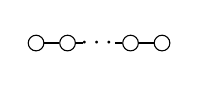
\begin{tikzpicture}[scale=0.4, baseline=-3pt, circ/.style={draw, circle, inner sep=2pt}]
        \node[circ] (1) at (0,0) {}; \node[circ] (2) at (1,0) {}; \node (3) at (2,0) {$\cdots$}; \node[circ] (4) at (3,0) {}; \node[circ] (5) at (4,0) {};
        \draw (1)--(2) (2)--(1.5,0) (2.5,0)--(4) (4)--(5);
    \end{tikzpicture} & $SL_{n+1}, PGL_{n+1}$ \\
    
    % --- Type B ---
    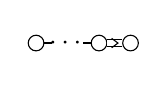
\begin{tikzpicture}[scale=0.4, baseline=-3pt, circ/.style={draw, circle, inner sep=2pt}]
        \node[circ] (1) at (0,0) {}; \node (2) at (1,0) {$\cdots$}; \node[circ] (3) at (2,0) {}; \node[circ] (4) at (3,0) {};
        \draw (1)--(0.5,0) (1.5,0)--(3);
        \draw[double, double distance=2pt] (3) -- (4);
        \draw (2.4,0.15) -- (2.6,0) -- (2.4,-0.15); % Arrow
    \end{tikzpicture} & $SO_{2n+1}$ \\

    % --- Type D ---
    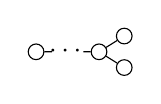
\begin{tikzpicture}[scale=0.4, baseline=-3pt, circ/.style={draw, circle, inner sep=2pt}]
        \node[circ] (1) at (0,0) {}; \node (2) at (1,0) {$\cdots$}; \node[circ] (3) at (2,0) {}; \node[circ] (4) at (2.8,0.5) {}; \node[circ] (5) at (2.8,-0.5) {};
        \draw (1)--(0.5,0) (1.5,0)--(3) (3)--(4) (3)--(5);
    \end{tikzpicture} & $SO_{2n}$ \\

    % --- Type E6 ---
    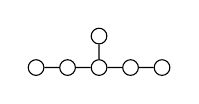
\begin{tikzpicture}[scale=0.4, baseline=-3pt, circ/.style={draw, circle, inner sep=2pt}]
        \node[circ] (1) at (0,0) {}; \node[circ] (2) at (1,0) {}; \node[circ] (3) at (2,0) {}; \node[circ] (4) at (3,0) {}; \node[circ] (5) at (4,0) {}; \node[circ] (6) at (2,1) {};
        \draw (1)--(2)--(3)--(4)--(5) (3)--(6);
    \end{tikzpicture} & $E_6$ \\

    % --- Type G2 ---
    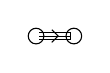
\begin{tikzpicture}[scale=0.4, baseline=-3pt, circ/.style={draw, circle, inner sep=2pt}]
        \node[circ] (1) at (0,0) {}; \node[circ] (2) at (1.2,0) {};
        \draw (1.1,0.1) -- (1.1,-0.1); % Triple line hack or use arrows
        \draw (1.1,0) -- (0.1,0); \draw (1.1,0.1) -- (0.1,0.1); \draw (1.1,-0.1) -- (0.1,-0.1);
        \draw (0.5,0.2) -- (0.7,0) -- (0.5,-0.2); % Arrowhead
    \end{tikzpicture} & $G_2$ \\
\end{tabular}
\fi
\newpage


\bibliographystyle{plain}
\bibliography{references.bib}

\end{document}